% Chapter 2

\chapter{Foundations and Concepts} % Write in your own chapter title
\label{Chapter2}
\lhead{Chapter \ref{Chapter2}. 
\emph{Foundations and Concepts}} % Write in your own chapter title to set the page header

{\bf \small{
This chapter presents\dots
}}


\section{Introduction}
% what is machine learning
% machine learning is in the peak ot its popularity and we can find it everywhere

% the goal is to find the underlying function that explains some phenomenon, which would help us predict new events

% supervised vs unsupervised 

% linear regression is one typical example, often used in science

% two of the most popular families of ML methods are: kernel methods and neural networks

% kernel methods advantages, theory, convexity; disadvantes: scalability

% neural networks advantages: scalability, flexibility; disadvantages: lack of theory



\section{Kernels and Implicit Features}
% los kernels son centrales en ML
Kernels are central in \acrshort{ml}, and some of the most successful methods use them, such as \acrshort{svms} or \acrshort{gps}.
The main advantage of using kernels, as we will see, is that we can send our data to a high, even infinite, dimensional space, where the problems of interest, regression or classification, are expected to be easier. Moreover, this transformation is made implicitly by exploiting the reproducing property of the kernels. This is named the kernel trick, and we will explain more carefully later in this section.

% están relacionados con la VC dimension porque nos permiten  
By using kernels, we change our feature space, from a finite-dimensional one to a much larger one, with possibly infinite dimensions. Although this might ease the problem of learning a function that explains our data, we also can encounter some problems. One is the curse of dimensionality, that is, the cost of finding a solution to optimization problems typically scales super-linearly with the dimension of our data. Other problem is overfitting, when the data is placed in a high-dimensional space the hypothesis that can explain the data are more expressive, and if they fit too exactly to the training data, they could not generalize well to new data. However, as we will see later in this Chapter, these problems can be solved.


\subsection{Learning in Feature Spaces} %

\begin{figure}[t!]
    \centering
    \subfloat[][Simplified \fdata{iris} example.]{%    
    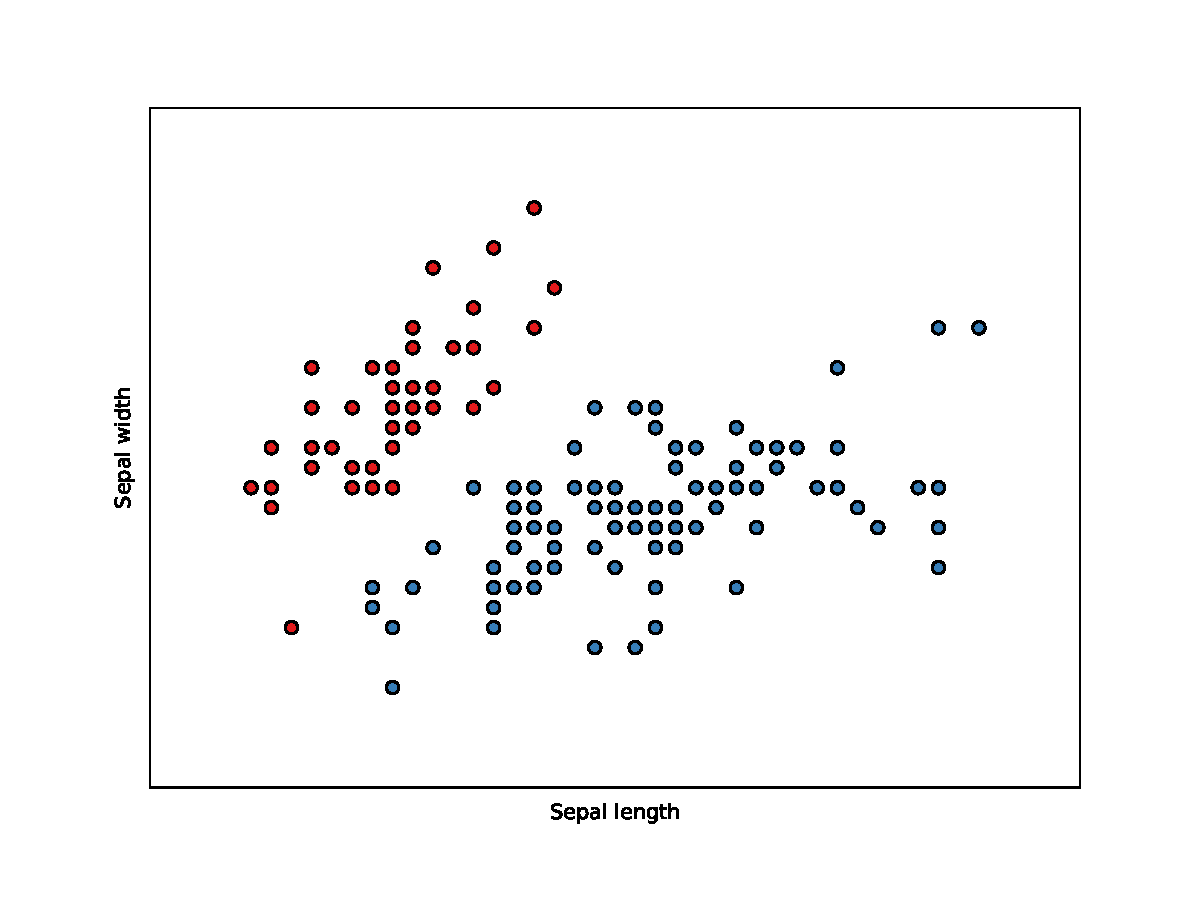
\includegraphics[width=0.45\textwidth]{Chapter2/Iris/iris.pdf}
    \label{fig:iris_example}}\quad%
    \subfloat[][Projections of simplified \fdata{iris} example.]{%
    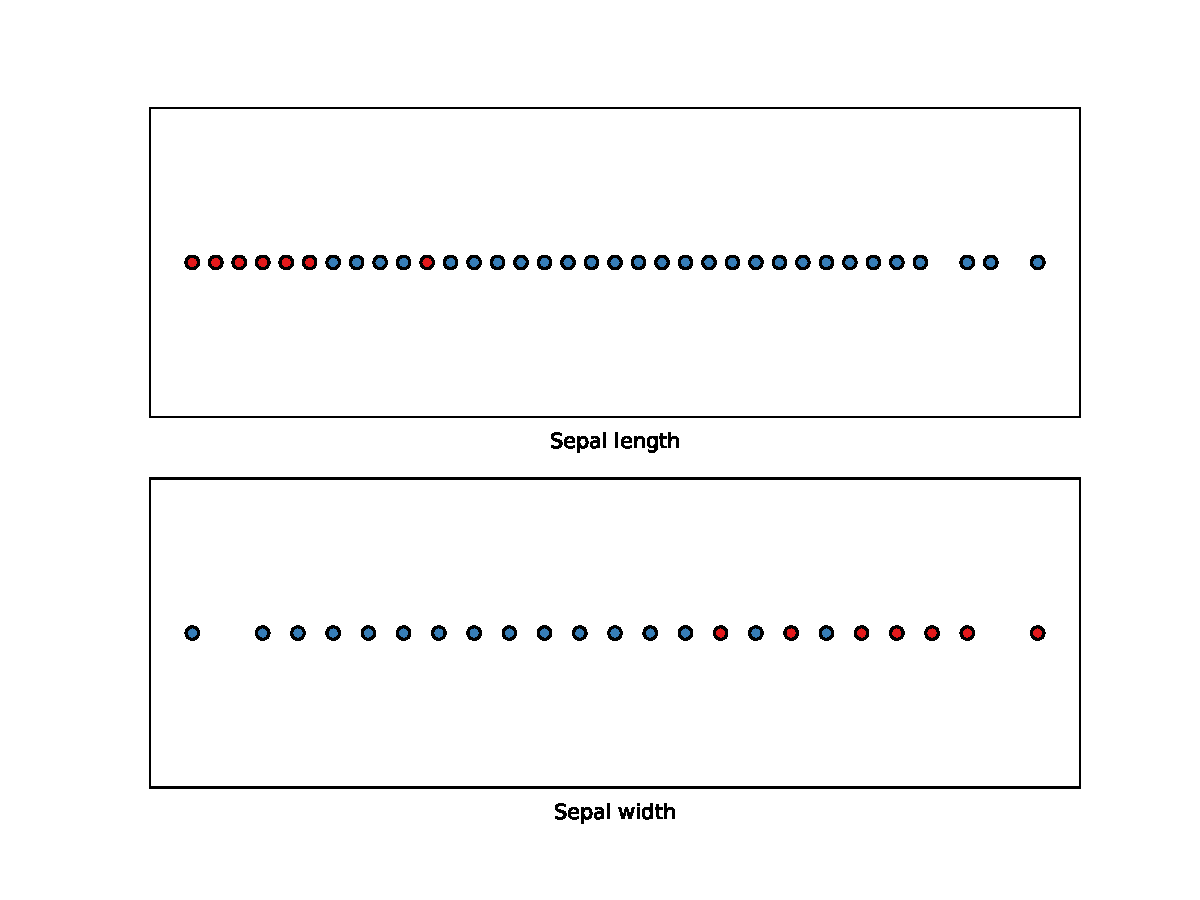
\includegraphics[width=0.45\textwidth]{Chapter2/Iris/projections_iris.pdf}
    \label{fig:iris_projections}}\\
    \caption{}
    \label{fig:iris}
\end{figure}

\begin{figure}[t!]
    \centering
    \subfloat[][Cubic regression problem. The underlying function, $f(x) = x^3$ is shown in orange, and the target values are the dots in blue.]{%    
    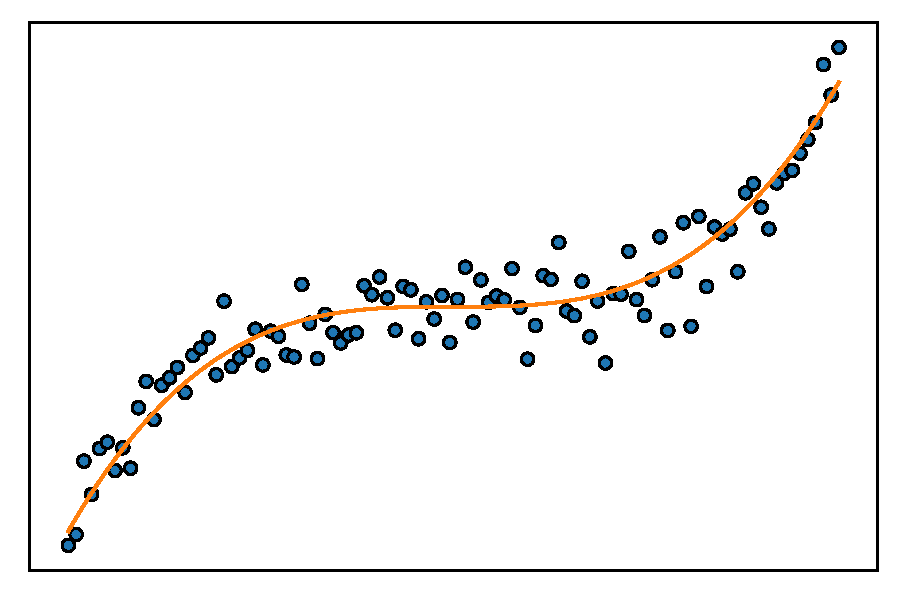
\includegraphics[width=0.3\textwidth]{Chapter2/CubicReg/regression_problem.pdf}
    \label{fig:cubicreg_example}}\quad%
    \subfloat[][Predictions with a linear feature space, including only $x$. The real function $f(x)=x^3$ is shown in orange and the predictions are the blue dots.]{%
    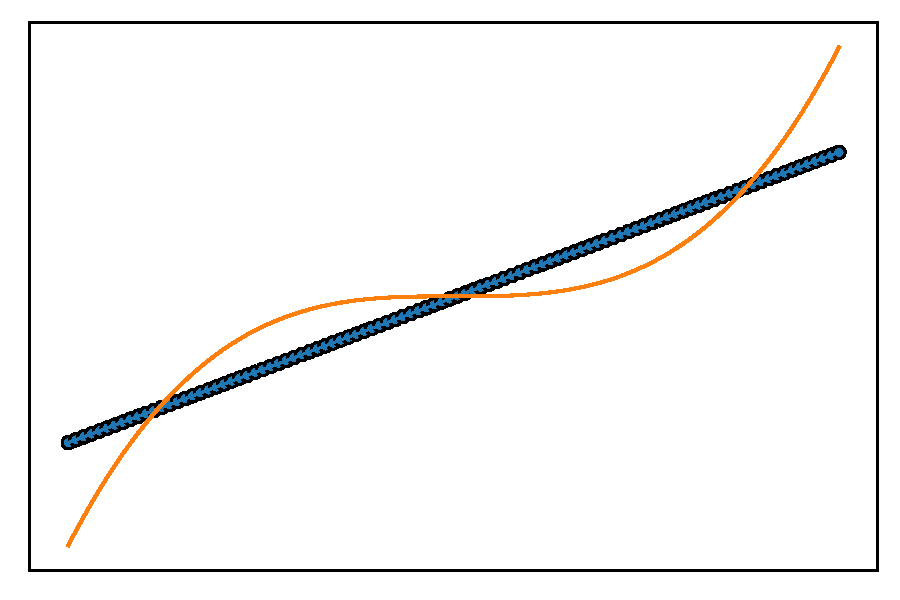
\includegraphics[width=0.3\textwidth]{Chapter2/CubicReg/regression_linearsol.pdf}
    \label{fig:cubicreg_linearsol}}\quad
    \subfloat[][Predictions with an extended feature space, including $x, x^2$ and $x^3$. The real function $f(x)=x^3$ is shown in orange and the predictions are the blue dots.]{%
    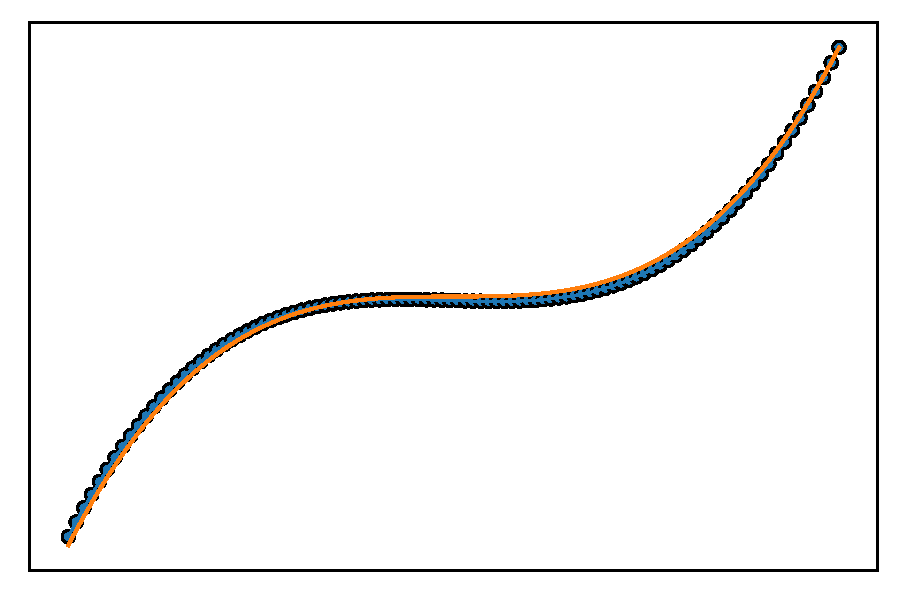
\includegraphics[width=0.3\textwidth]{Chapter2/CubicReg/regression_cubicsol.pdf}
    \label{fig:cubicreg_cubicsol}}
    \\
    \caption{}
    \label{fig:cubicreg}
\end{figure}

In \acrshort{ml} the choice of the feature space is crucial. If it is too small or too poor, it is not possible to find a good solution to our problem.
Consider the classification setting, when the feature space is low-dimensional, the classed are more overlapped and finding a decision boundary is more challenging. 
%
Take for example the popular \fdata{iris} dataset, where the goal is to discriminate between three species of iris flowers: \emph{setosa}, \emph{virginica} and \emph{versicolor}. To do this, $50$ samples from each species are gathered, and four features are measured for each sample: the length and width of the petals and of the sepals.
%
Now, for illustration purposes, we take a simplified version in which the goal is to discriminate the \emph{setosa} class from the rest, and where we consider only two features: the length and width of the sepals. In Figure~\ref{fig:iris_example} we represent the data corresponding to this simplified version of the \fdata{iris} problem, and we can observe that the two clouds of points are easily separable by a linear function. However, if, instead of the two-dimensional space, we consider just one feature, the problem is no longer separable. In Figure~\ref{fig:iris_projections} we note that the two classes are no longer separable.
%

For an example of how enlarging the feature space can lead to better solutions, consider a regression problem where we take $100$ one-dimensional points linearly distributed in the feature space, in this case $[-2, 2]$; then we compute the target values as $y_i = x_i^3 + \epsilon_i$, where $\epsilon_i \sim \normal{0, 1}$. This is a regression problem that we illustrate in Figure~\ref{fig:cubicreg_example}. If we consider a linear regression model with the original feature space, it will not be able to approximate well the function $f(x)=x^3$, and the solution is depicted in Figure~\ref{fig:cubicreg_linearsol}.
However, if we enlarge the feature space using the transformation $\phi(\cdot)$ defined as
\begin{equation}
    \begin{aligned}
        \nonumber
        \phi:\Xspace &\to\Xspace^3 \\
        x &\to (x, x^2, x^3) ,
    \end{aligned}
\end{equation}
then a linear regression model in this new space can find a good approximation, as the one shown in Figure~\ref{fig:cubicreg_cubicsol}.
%

This kind of result is one of the motivations for using kernels. 
As we will see later, the linear formulations, such as the Linear Regression or \acrshort{svms}, has a dual formulation, which does not depend directly on the features $x_i$, but on the inner products $\dotp{x_i}{x_j}$.
Consider now that we have the feature space $\Xspace = \reals^2$, and we consider the following function:
\begin{equation}
    \begin{aligned}
        \nonumber
        k: & &\reals^2 \times &\reals^2 & &\to& &\reals \\
        & &((x_1, x_2), & (y_1, y_2))   & &\to& ((x_1, x_2)^\intercal &(y_1, y_2) + c)^2 .
    \end{aligned}
\end{equation}
Now, we can observe the following fact:
\begin{equation}
    \nonumber
    \begin{aligned}
        &((x_1, x_2)^\intercal (y_1, y_2) + c)^2 \\
        &= \left(x_1 y_1 + x_2 y_2 + c \right)^2 \\
        &= x_1^2 y_1^2 + 2 x_1 y_1 x_2 y_1+ x_2^2 y_2^2 + 2 c x_1 y_1 + 2 c x_2 y_2 + c^2 \\
        &= \dotp{(c, \sqrt{2c} x_1, \sqrt{2c} x_2, \sqrt{2} x_1 x_2, x_1^2, x_2^2)}{(c, \sqrt{2c} y_1, \sqrt{2c} y_2, \sqrt{2} y_1 y_2, y_1^2, y_2^2)}.
        %&= \dotp{\psi((x_1, x_2))}{\psi((y_1, y_2))} .
    \end{aligned}
\end{equation}
Therefore, if we have a model that depends on the inner products of the data in our feature space $x, y \in \Xspace$, and we define these inner products as $k(x, y) = (x^\intercal y + c)^2$, we are implicitly enlarging the feature space with the transformation $\psi$, defined as
\begin{equation}
    \begin{aligned}
        \nonumber
        \psi: & &&\reals^2 & &\to& &\reals^6 \\
        & &(x_1,& x_2)& &\to& (c, \sqrt{2c} x_1, \sqrt{2c} x_2,& \sqrt{2} x_1 x_2, x_1^2, x_2^2) ,
    \end{aligned}
\end{equation}
such that $k(x, y) = \dotp{\psi(x)}{\psi(y)}$.
%
Here, the function $k(\cdot, \cdot)$ is a kernel function, in particular, this is the polynomial kernel, and $\psi(\cdot)$ is its associated feature transformation. 
We remark that in the dual formulation of linear models, which will be explained in detail later, all we need is to define a proper kernel function that must meet some requirements, and, as we will see, it has an associated feature transformation function; then, by defining the kernel function, we are implicitly enlarging our feature space.




% linear models use the original space
% low-dimensional data is more interpretable but less expresive: there exists feature selection techniques
% high-dimensional data is less interpretable but more expressive
% ejemplo de problema no lineal (cuadrático o cúbico de clasificación) no lineal y usar kernel polinómico
% esto es un kernel, y es útil porque podemos resolver los problemas más facilmente

\subsection{The Reproducing Kernel Map} % three characterizations
% rkhs
To make use of kernels and to ensure that they have a corresponding feature transformation function that extends our feature space, we have to define some concepts and give some previous results.
In first place, we define the inner product.
%
\begin{definition}[Inner Product]
    An inner product on vector space $\Vspace$ is a map
    $$\dotp{\cdot}{\cdot}: \Vspace \times \Vspace \to \reals , $$
    that for all $u, v, w \in \Vspace$ and $a, b \in \reals$ satisfy:
    \begin{enumerate}
        \item $\dotp{u}{a v + b w} = a\dotp{u}{v} + b\dotp{u}{w}$ (linear);
        \item $\dotp{u}{v} = \dotp{v}{u}$ (symmetric) ;
        \item $\dotp{u}{u} \geq 0, \; \dotp{u}{u} = 0 \implies u = 0$ (positive definite) .
    \end{enumerate} 
\end{definition}
%
Then, we define a positive definite kernel function, which has some similarities with the inner product.
\begin{definition}[Positive Definite Kernel]
    Given a non-empty set $\Xspace$, a symmetric function
    \begin{equation}
        \nonumber
        k: \Xspace \times \Xspace \to \reals
    \end{equation}
    is a positive definite kernel if for any set $x_1, \ldots, x_\nsamples \in \Xspace$ and $c_1, \ldots, c_\nsamples \in \reals$,
    \begin{equation}
        \nonumber
        \sum_{i=1}^\nsamples \sum_{j=1}^\nsamples c_i c_j k(x_i, x_j) \geq 0 ,
    \end{equation} 
    and if $\sum_{i=1}^\nsamples \sum_{j=1}^\nsamples c_i c_j k(x_i, x_j)$, then $c_1, \ldots, c_n = 0$.
\end{definition}
%
It can be seen that both the inner product and the kernel function are symmetric and positive-definite. The connection between both goes further, and we will see it below.
%
For simplicity, we will say positive kernel or just kernel instead of positive definite kernel. We can characterize a kernel also using finite sets and the corresponding matrices built using such kernel. To do this we need to define the Gram (or kernel) matrix and positive definite matrix first.
%
\begin{definition}[Gram Matrix]
    Given a symmetric function
    \begin{equation}
        \nonumber
        k: \Xspace \times \Xspace \to \reals
    \end{equation}
    and patterns $x_1, \ldots, x_\nsamples$, the matrix $\fm{K}$ with elements $\fm{K}_{ij} = k(x_i, x_j)$, with $i,j=1, \ldots, n$, is called the Gram matrix.
\end{definition}
%
\begin{definition}[Positive Definite Matrix]
    A matrix $K \in \reals^{n \times n}$ is positive definite if
    $\sum_{i=1}^n \sum_{i=1}^n K_{ij} c_i, c_j \geq 0$ 
    for any $c_1, \ldots, c_n \in \reals$ and if $\sum_{i=1}^n \sum_{i=1}^n K_{ij} c_i, c_j = 0$, then $c_1, \ldots, c_n = 0$.
\end{definition}
%
Then, it is easy to characterize a kernel function by its kernel matrices, as stated in the following lemma.
%
\begin{lemma}
    Given a non-empty set $\Xspace$, a symmetric function
    \begin{equation}
        \nonumber
        k: \Xspace \times \Xspace \to \reals
    \end{equation}
    is a positive definite kernel if for any set $x_1, \ldots, x_\nsamples \in \Xspace$ and $c_1, \ldots, c_\nsamples \in \reals$, the corresponding Gram matrix is positive definite.
\end{lemma}
%

As illustrated in the previous subsection, we are interested in using kernels to implicitly transform our data. Consider the map from $\Xspace$, a non-empty set, into the space of functions $f: \Xspace \to \reals$, which we denote as $\reals^\Xspace$, defined as 
    \begin{equation}
        \begin{aligned}
            \nonumber
            \phi: \Xspace &\to \reals^\Xspace \\
            x &\to k(\cdot, x) .
        \end{aligned}
    \end{equation}
Here, we are transforming each point $x$ into a function that assigns the value $\phi(\tilde{x}) = k(\tilde{x}, x)$ to every $\tilde{x} \in \Xspace$. That is, in the new space, $x$ is defined by its similarity, expressed by $k(\tilde{x}, x)$, to every other points $\tilde{x} \in \Xspace$. This transformation seems difficult to work with because our new features are functions.
However, we can define a feature space associated with $\phi$, with an inner product associated with the kernel function $k(\cdot, \cdot)$. To do this, we follow three steps: we Define a vector space from the image of $\phi$, define an inner product in such space, and show that this inner product satisfies $\dotp{\phi(\tilde{x})}{\phi(x)} = k(\tilde{x}, x)$.
We begin by considering all linear combinations of images of $\phi$, that is, the functions 
$$ f(\cdot) = \sum_{i=1}^n \alpha_i \phi(x_i) =\sum_{i=1}^n \alpha_i k(\cdot, x_i), $$
with $\alpha_1, \ldots, \alpha_n \in \reals$.
The set of such functions is a vector space $\Vspace_\phi \subset \reals^\Xspace$, since given other function 
$$ g(\cdot) = \sum_{i=1}^m \beta_i \phi(\tilde{x}_i) =\sum_{i=1}^n \beta_i k(\cdot, \tilde{x}_i) ,$$
with $\beta_1, \ldots, \beta_m \in \reals$,
we have that $f(\cdot) + g(\cdot) \in \Vspace_\phi$, and for any $a \in \reals$,  $a f(\cdot) \in \Vspace_\phi$.
Now, we can define an inner product in this vector space as 
$$ \dotp{f(\cdot)}{g(\cdot)} = \sum_{i=1}^n \sum_{i=1}^m \alpha_i \beta_j k(x_i, \tilde{x}_j),$$
and we have to check that it satisfies the properties of an inner product. It is easy to see its linearity, since it is a sum, and the symmetry property holds from the symmetry of the kernel function. Finally, to check that it is positive definite we observe that because $k(\cdot, \cdot)$ is positive definite,
$$ \dotp{f(\cdot)}{f(\cdot)} = \sum_{i=1}^n \sum_{j=1}^n \alpha_i \alpha_j k(x_i, x_j) \geq 0$$
for any $x_1, \ldots, x_n \in \Xspace$ and $\alpha_1, \ldots, \alpha_n \in \reals$, and if $\dotp{f(\cdot)}{f(\cdot)} = 0$, then $\alpha_1, \ldots, \alpha_n =0$, hence $f(\cdot) = 0$.
%
This inner product is defined for any pair of functions $f(\cdot), g(\cdot) \in \Vspace_\phi$, in particular, consider $g(\cdot) = \phi(\tilde{x}) = k(\cdot, \tilde{x})$, then, from the definitions, we have that
$$ \dotp{f}{k(\cdot, \tilde{x})} = \sum_{i=1}^n \alpha_i \phi(x_i) =\sum_{i=1}^n \alpha_i k(x_i, \tilde{x}) = f(\tilde{x}) .$$
That is, $k(\cdot, \tilde{x})$ is the representative of the evaluation on $\tilde{x}$. Moreover, we observe that with $f(x) = \phi(x)$,
$$ \dotp{\phi(x)}{\phi(\tilde{x})} = \dotp{k(\cdot, x)}{k(\cdot, \tilde{x})} = k(x, \tilde{x}) .$$  
This is the reproducing property of the kernel, and it defines an easy way of computing inner products in the feature space of functions $\reals^\Xspace$, to compute the inner product between $\phi(x)$ and $\phi(\tilde{x})$, we just need to compute the kernel value $k(x, \tilde{x})$.

\subsection{Reproducing Kernel Hilbert Spaces}
%
Kernels, with its reproducing property, have a close connection with a particular class of Hilbert spaces, which are named \acrfull{rkhss}. First, we give the definition of Hilbert space.
%
\begin{definition}[Hilbert Space]
    A Hilbert space is a vector space $\hilbertspace$ with an inner product $\dotp{\cdot}{\cdot}$, such that under the norm defined by $\norm{u} = \sqrt{\dotp{u}{u}}, \; u \in \hilbertspace$, it is a complete metric space.
\end{definition}
%
An example of Hilbert space is $\reals^d$ with the inner product defined as $\dotp{u}{v} = u^\intercal v$.
%
% The completeness of a space can be defined in terms of the convergence of its Cauchy sequences, but, for the goals of this work, we can omit the details. 
We are interested in drawing the connection between kernels and the \acrshort{rkhss}, which is given in the following definition.
\begin{definition}[\acrshort{rkhs}]
    Given a non-empty set $\Xspace$, a Hilbert space $\hilbertspace$ of functions $f: \Xspace \to \reals$ with an inner product $\dotp{\cdot}{\cdot}$ is an \acrshort{rkhs} if there exists a symmetric function $k: \Xspace \times \Xspace \to \reals$ such that $\dotp{f}{k(x, \cdot)} = f(x)$ for all $f \in \hilbertspace$, and $\overline{\Span{\set{k(\cdot, x), x \in \Xspace}}} = \hilbertspace$. 
\end{definition}
Here, $\Span{\set{k(\cdot, x), x \in \Xspace}}$ is the span of functions $k(\cdot, x)$, that is functions defined as
$$ f(\cdot) = \sum_{i=1}^n \alpha_i \phi(x_i) =\sum_{i=1}^n \alpha_i k(\cdot, x_i), $$
and $\overline{\mathcal{A}}$ is the completion of set $\mathcal{A}$, which include the set itself and the limits of all its Cauchy sequences.
Other way to characterize \acrshort{rkhss} is as the Hilbert spaces $\hilbertspace$ with continuous evaluation functionals, the maps
\begin{equation}
            \begin{aligned}
        \nonumber
        E_{x}: \hilbertspace &\to \reals \\
        f &\to f(x) .
    \end{aligned}
\end{equation}
In this case, according to the Riesz Theorem~\citep{Whittaker1991ACI}, for every $x \in \Xspace$ there exists a single $g_x \in \hilbertspace$ such that
$$ E_x(f) = \dotp{f}{g_x}, \; \forall f \in \hilbertspace.$$
In particular, for $f = g_{\tilde{x}}$ we have $E_x(g_{\tilde{x}}) = g_{{\tilde{x}}}(x) = \dotp{g_x}{g_{\tilde{x}}}$. If we define a function $k(x, \tilde{x}) = \dotp{g_x}{g_{\tilde{x}}}$, then we can see that it is a reproducing kernel. It is symmetric because of the symmetry of the inner product, and definite positive because the inner product is also positive definite. The reproducing property 
hold from the definitions if we consider $k(\cdot, x) = g_x$.
%
Observe that, given an \acrshort{rkhs}, a Hilbert space with continuous evaluation functionals, it defines a unique kernel that is the reproducing kernel for such space, where the uniqueness comes from the unique evaluation representatives in the Riesz Theorem.
%

It is also possible to prove the converse, that is, given a positive definite kernel function, there exists an associated \acrshort{rkhs}.
To do that we need to generate a Hilbert space from a kernel function, which is done by considering its associated integral operator, whose properties are expressed in the Mercer theorem. In this theorem we use some concepts of measure theory. 
%
Given a non-empty set $\Xspace$, we consider a measurable space $(\Xspace, \mu)$ where $\mu$ is the measure. The expression ``almost everywhere'' means in every subset $\mathcal{S} \subset \Xspace$ such that $\mu(\mathcal{S}) \neq 0$. We also use the formulation $L_2(\Xspace)$ for the functions $f: \Xspace \to \reals$ that are measurable, that is,
$$ \int_{\Xspace} f(x) d\mu(x) < \infty .$$

\begin{definition}[Mercer Kernel]
    Let $k: \Xspace \times \Xspace \to \reals$ a symmetric continuous function, such that the integral operator 
    \begin{equation}
        \begin{aligned}
    \nonumber
    T_k: L_2(\Xspace) &\to L_2(\Xspace) \\
    f &\to \int_\Xspace k(x, \tilde{x}) f(x) d \mu(\tilde{x}) 
\end{aligned}
\end{equation}    
is positive definite; that is; for any $f \in L_2(\Xspace)$, 
\begin{equation}
    \nonumber
    \int_{\Xspace \times \Xspace} k(x, \tilde{x}) f(x) f(\tilde{x}) d\mu(x) d\mu(\tilde{x}) \geq 0 ,
\end{equation}
then $k$ is a Mercer kernel
\end{definition}

\begin{theorem}[Mercer Theorem]    
Let $k$ be a Mercer kernel and consider the normalized eigenfunctions $\psi_i \in L_s(\Xspace)$ and associated eigenvalues $\lambda_i$ of the operator $T_k$, such that
$$ T_k(\psi_i) = \lambda_i \psi_i , $$
then $\lambda_i > 0$ and $k(x, \tilde{x}) = \sum_{i=1}^\infty \lambda_i \psi_i(x) \psi_i(\tilde{x})$ almost everywhere, where the eigenvalues $\lambda_i$ are sorted in non-increasing order. 
\end{theorem}
%
With this result, we can construct a Hilbert space whose reproducing kernel is $k$.
Consider the following feature transformation
\begin{equation}
    \begin{aligned}
        \nonumber
        \phi: \Xspace &\to l_2 \\
        x &\to \left(\sqrt{\lambda_1} \psi_1(x), \sqrt{\lambda_2} \psi_2(x), \ldots \right) ,
    \end{aligned}
\end{equation}
where $l_2$ is the space of all sequences $(x_n)_{n \in \naturals}$ such that $$ \sum_{n \in \naturals} x_n < \infty .$$
In this space, the inner product between $\phi(x)$ and $\phi(\tilde{x})$ is defined as
$$ \dotp{\phi(x)}{\phi(\tilde{x})} = \sum_{i=1}^\infty \lambda_i \psi_i(x) \psi_i(\tilde{x}),$$ which, by the Mercer theorem, is equivalent to saying that $\dotp{\phi(x)}{\phi(\tilde{x})} = k(x, \tilde{x})$.

Therefore, we have seen that there is a one-to-one correspondence between positive definite kernels and \acrshort{rkhss}. Given an \acrshort{rkhs} there is a single kernel function that has the reproducing property in that space. Also, given a positive definite kernel $k$, there exists an associated \acrshort{rkhs} such that $k$ is its reproducing kernel. 

% mercer theorem?

% kernels as a measure of distance
% ejemplo de kernel Gaussiano e implicit transformation









\section{Risk and Regularization}
To automatize the learning process, which is the goal of \acrshort{ml}, it is necessary to define a criterion to measure the performance of the functions $f: \Xspace \to \Yspace$ estimated from the data.
At each particular sample $(x_i, y_i)$ we can give a metric of how close we are to our desired goal, this is the selected loss function. If we have a classification problem, we may want to minimize the number of incorrectly classified patterns, but this quantity is not differentiable and not easy to work with. In regression problems, we would like to minimize the distance between the regression function and the training target values, but there are also multiple ways to define this distance. 
%

Anyway, independently of the chosen loss function, the data that we use have been sampled, and we do not know the distribution. There are some samples more important than others, because they belong to an area of high probability, according to this unknown distribution. Getting a bad result, as defined by the loss function, in a sample that is an outlier of the distribution is not that relevant, because few data is expected to be sampled in its neighborhood. 
To account for this, we define the expected risk, which we want to minimize. Nevertheless, since the distribution is unknown, we consider it in an implicit way by minimizing the empirical risk.

%
However, when minimizing the empirical risk instead of the expected one, we might find that we are too influenced by the particular sample that we have been given.  If the training data is too scarce, or also if we have some prior knowledge that we want to incorporate to the learning process, the regularization of the models can be helpful, as we will describe.
%
Moreover, when we use linear models to minimize his regularized risk, there is a result that describes the solution in terms of the training data, which is crucial for kernel methods, especially where the linear model is built in an infinite dimensional space.

\subsection{Loss Functions}
Given a feature space $\Xspace$ and a target space $\Yspace$, the criterion that we use to measure the performance of our estimates $f: \Xspace \to \Yspace$ is defined by the loss functions.
Here, we give the definition of loss function and present the losses that we will use in the rest of this work.

\begin{definition}[Loss Function]
    Denote $(y, f(x))$ as the pairs consisting on an observation $y \in \Yspace$ and a prediction $f(x) \in \Yspace$, with $x \in \Xspace$ an element of the feature space, then any map
    \begin{equation}
        \begin{aligned}
    \nonumber
    \lossf: &\Yspace \times \Yspace &\to &&[0, \infty) \\
    &(y, f(x)) &\to  && \lossf(y, f(x)) 
\end{aligned}
\end{equation}
  %  $$ \lossf: \Yspace \times \Yspace \to [0, \infty)$$    
    such that $\lossf(y, y) = 0$ for all $y \in \Yspace$ is a loss function.
\end{definition}
Observe that $\lossf(\cdot, \cdot)$ is a non-negative function and the perfect prediction always achieves its minimum value.

% Classification
In the binary classification problems, if we want to minimize the number of misclassified patterns, we use the \emph{accuracy} loss, which, with the labels $\set{0, 1}$ for the classes, is defined as
\begin{equation}
    \nonumber
    \lossf(y, f(x)) = (y - f(x))^2 =
    \begin{cases}
        0, & y = f(x) ,\\
        1, & y \neq f(x) .
    \end{cases}
\end{equation}
However, this function only takes into account if the example is correctly classified or not, but we might also want to take into account the confidence that we have in this decision. If we use the labels $\set{-1, 1}$ to denote the two classes, then we can look at the number $y f(x)$ to check if the decision is correct, only if $y f(x) > 0$ the pattern is correctly classified. That is, we are looking at a single value to determine the success of our decision, and we can also use it to define a confidence. For example, we can consider that in those patterns where $0 < y f(x) < 1$, although correctly classified, the confidence that we have to make such decision is not enough, and only when $y f(x) \geq 1$ we consider that it is a correct classification. We can interpret this as a confidence margin, and the loss function that implements this is called \emph{soft margin}, or also \emph{hinge} loss, which is defined as
\begin{equation}
    \label{eq:hinge_def}
    \lossf(y, f(x)) = \pospart{1 - yf(x)} = 
    \begin{cases}
        0, & y f(x) \geq 1 ,\\
        1 - y f(x), & y f(x) < 1 .
    \end{cases}
\end{equation}
This is a continuous function where we can observe two charactistics. One is confidence margin where we ask $y f(x) \geq 1$ to consider it a decision without penalization. The other, is that the penalization grows linearly as $y f(x)$ decreases.
%
A modification of the hinge loss considers the same margin, but the penalization for the misclassified patterns grows as a quadratic function. This is the \emph{squared hinge} loss, whose expression is
\begin{equation}
    \label{eq:sqhinge_def}
    \lossf(y, f(x)) = \pospart{1 - yf(x)}^2 = 
    \begin{cases}
        0, & y f(x) \geq 1 ,\\
        (1 - y f(x))^2, & y f(x) < 1 .
    \end{cases}
\end{equation}
%
Finally, another commonly used function is the \emph{logistic loss}, where the classes are labeled as $\set{0, 1}$. With this loss, we model $P(y=1 \vert x)$, that is, the probability of $x$ being a pattern from class $1$, by using the sigmoid function $s(\cdot)$ as 
$$ s(f(x)) = \frac{1}{1 + \exp{(-f(x))}} .$$
Here, although $f(x) \in \reals$, $s(f(x)) \in (0, 1)$, so we can see it as the probability of being from class $1$. Then, the loss function is defined as 
\begin{equation}
    \label{eq:logistic_def}
    \lossf(y, f(x)) = - y \log{(s(f(x)))} - (1 - y) \log{(1 - s(f(x)))} .
\end{equation} 
Here, given for example a pattern from class $y=1$, only the first term is active, and the larger $f(x)$ is, the closer $s(f(x))$ gets to $1$, so the penalization is smaller.
In the binary classification scenario, the \emph{logistic} loss resembles the \emph{hinge} one. 

The formulae~\eqref{eq:logistic_def} also looks like the definition of entropy, so it is also named \emph{cross-entropy} loss. 
With the entropy interpretation, this loss is easily adaptable to the multi-class case with classes $\set{1, \ldots, C}$. Consider the one-hot encoding vector $\fv{y}$ of length $C$, such that $\fv{y}_c = 1$ if $y=c$ and $\fv{y}_c = 0$ otherwise, for $c=1, \ldots, C$.
Now, we can model the probabilities $P(y=c \vert x) = f_c(x)$ with $c \in \set{1, \ldots, C}$ and form the corresponding vector $\fv{f}(x)$; then, the multi-class \emph{cross-entropy} loss is defined as 
\begin{equation}
    \label{eq:crossentropy_def}
    \lossf(\fv{y}, f(x)) = - \sum_{c=1}^C \fv{y}_i \log{(s(\fv{f}_i(x)))} .
\end{equation} 
For the rest of loss functions there are also proposals for extending them to the multi-class case, but we will not use them in this work.

%Regression
In the regression problems, given a pair $(x, y) \in \Xspace \times \Yspace$, the goal is to minimize the distance between the observed target $y$ and our prediction $f(x)$; then, a natural loss is the \emph{absolute} loss function, defined as 
\begin{equation}
    \label{eq:abs_def}
    \lossf(y, f(x)) = \abs{y - f(x)}.
\end{equation}
Here, any mistake is penalized, but there might be some cases when the targets are noisy, so we would like to have some room for small errors. Concretely, if $f(\cdot)$ is the perfect regression function, the target values might be $y = f(x) + z$ with $z \sim \normal{0, \sigma}$; then, it might be not sensible to not penalize those errors that can be explained by this noise. This is done in the \emph{$\epsilon$-insensitive} loss function, which is expressed as 
\begin{equation}
    \label{eq:epsins_def}
    \lossf(y, f(x)) = \abs{y - f(x)}_\epsilon =
    \begin{cases}
        0, & \abs{y - f(x)} \leq \epsilon ,\\
        \abs{y - f(x)} - \epsilon, & \abs{y - f(x)} > \epsilon .\\
    \end{cases}
\end{equation} 
Here, $\epsilon$ is a hyperparameter and have to be selected for each specific problem. Also, observe that with $\epsilon =0$, we have the \emph{absolute} loss.
%
The regression losses presented are based on the absolute value $\abs{y - f(x)}$, thus, they are not differentiable. One alternative is to use the squared value of the distance, as expressed in the \emph{squared} loss:
\begin{equation}
    \label{eq:sq_def}
    \lossf(y, f(x)) = (y - f(x))^2.
\end{equation}
% and, analogously, the \emph{squared $\epsilon$-insensitive} loss, defined as
% \begin{equation}
%     \label{eq:epsins_def}
%     \lossf(y, f(x)) = 
%     \begin{cases}
%         0, & \abs{y - f(x)} \leq \epsilon ,\\
%         \abs{y - f(x)} - \epsilon, & \abs{y - f(x)} > \epsilon .\\
%     \end{cases}
% \end{equation} 
The \emph{squared} loss is also easily adaptable to the multi-target regression problems. Consider the case with $K$ targets for each feature vector $x$, that is, $\fv{y}$ are vectors of length $K$, and we produce the corresponding vector of predictions $\fv{f}(x)$; then, the multi-target \emph{squared} loss is
\begin{equation}
    \label{eq:sqmulti_def}
    \lossf(y, f(x)) =  \norm{\fv{y} - \fv{f}(x)}^2.
\end{equation}
%
The $\epsilon$-insensitive loss can also be extended to use the squared value of the distance. The squared $\epsilon$-insensitive loss is defined as
\begin{equation}
    \label{eq:sqepsins_def}
    \lossf(y, f(x)) = \abs{y - f(x)}^2_\epsilon =
    \begin{cases}
        0, & (y - f(x))^2 \leq \epsilon ,\\
        (y - f(x))^2 - \epsilon, & (y - f(x))^2 > \epsilon .\\
    \end{cases}
\end{equation} 

\subsection{Empirical and Expected Risk} 
In \acrshort{ml}, we have a feature space $\Xspace$ and a target (or label) space $\Yspace$, and we believe that there is a function $f: \Xspace \to \Yspace$, and if we have a good estimate of such function, we will be able to predict new target values $y$ given a pattern $x$. 

%
We begin with the classification setting. Take for example the popular problem \fdata{MNIST} of handwritten digits, where the feature space $\Xspace$ is the space of $28 \times 28$ matrices with values in $[0, 1]$, corresponding to the pixels of $28 \times 28$ grayscale images, i.e. $[0, 1]^{28 \times 28}$. We believe that there exists a function $f: \Xspace \to \reals$ that captures the properties of the handwritten digit $0$ such that $f(x)=1$ only when $x$ is an image of digit $0$ and $f(x)=0$ otherwise. Then, we would like to learn such function, so when a new image $\tilde{x}$ comes in, we can automatically decide if it represents the digit $0$ by looking at the value $f(x)$.
%
We suppose that there exists a distribution for images of digits and its labels, such that $\distf(x, y=1) = \distf(x \vert y = 0) \distf(y = 1)$ captures the properties of the images of digit $0$. Then, our function $f$ then minimizes the expected accuracy
$$ \int_{\Xspace \times \Yspace} (y - f(x))^2 d\distf(x, y) ,$$
where we are using the \emph{accuracy} loss function $\ell(y, f(x)) = (y - f(x))^2$. 
%
If we want to consider other losses, such as the \emph{hinge} loss, we can consider that $\mathcal{Y} = \reals$, where the labels are encoded as $\set{-1, 1}$, the goal is to minimize 
$$ \int_{\Xspace \times \Yspace} \pospart{1 - y f(x)} d\distf(x, y) .$$

%
In the regression setting we find a similar situation. Consider the housing examples, where we want to predict the economic value of houses using descriptive features of each property: location, number of rooms, floor number, etc. These characteristics are our feature space $\Xspace$, and the output space is $\Yspace = \reals^+$, i.e. the positive real numbers, since we want to predict prices. Again, we suppose that the prices are dependent on the characteristics of each house, such that there exists a joint distribution $\distf(x, y)$.
Now, we want to find the function $f: \Xspace \to \Yspace$ that minimizes the expected \emph{squared} loss
$$ \int_{\Xspace \times \Yspace} (y - f(x))^2 d\distf(x, y) .$$
Observe that although the formula is the same as the one used for the accuracy loss in classification, here the output space $\Yspace$ is the positive reals, so it has a different meaning. Now, the function $f$ minimizing such quantity a good estimate to predict the value of a new property given its characteristics.

%
In both classification and regression cases, we arrive at an integral of a loss function.
This is called the expected risk, because we take the expectation of the loss function with respect to the real distribution of data. 
%
In general, in \acrshort{ml} we consider a set of hypothesis $\hypspace = \set{\hypf(\cdot, \param) \in \paramspace}$ where $\param$ are the parameters that define each hypothesis and $\paramspace$ is the space of such parameters. Then, the desired goal is to select the candidate hypothesis that minimizes the expected risk, which is defined as follows.
%
\begin{definition}[Expected Risk Minimization]
    Given the space $\Xspace \times \Yspace$ with a distribution $\distf(x, y)$ and a loss function $\ell$. Consider a set of hypothesis $\hypspace = \set{\hypf(\cdot, \param) \in \paramspace}$ parametrized by $\param \in \paramspace$, then the expected risk minimization problem is 
    \begin{equation}
        \label{eq:exprisk_def}
        \argmin_{\param \in \paramspace} \exprisk(\param) = \int_{\Xspace \times \Yspace} \ell(y, \hyp{x}{\param}) d\distf(x, y) .
    \end{equation}
\end{definition}
%
The distribution $\distf$ that appears in the expected risk is unknown, so it is not possible to find a solution to the minimization problem~\eqref{eq:exprisk_def}.
% 
Instead, what we have is a sample 
\begin{equation}
    \nonumber
    \sample = \set{(x_i, y_i), \; i=1, \ldots, \nsamples} ,
\end{equation}
where each pair $(x_i, y_i)$ have been independently sampled from $\distf(x, y)$. 
%
Then, we use this sample $\sample$ to define the empirical risk minimization problem.
%
\begin{definition}[Empirical Risk Minimization]
    Given the space $\Xspace \times \Yspace$ with a distribution $\distf(x, y)$ and a loss function $\ell$. Consider a set of hypothesis $\hypspace = \set{\hypf(\cdot, \param) \in \paramspace}$ parametrized by $\param \in \paramspace$, and a set 
    \begin{equation}
        \nonumber
        \sample = \set{(x_i, y_i), \; i=1, \ldots, \nsamples} ,
    \end{equation}
    of pairs $(x_i, y_i)$ independently sampled from $\distf(x, y)$;    
    then, the empirical risk minimization problem is 
    \begin{equation}
        \label{eq:emprisk_def}
        \argmin_{\param \in \paramspace} \emprisk(\param) = \frac{1}{\nsamples} \sum_{i=1}^\nsamples \ell(y_i, \hyp{x_i}{\param}) .
    \end{equation}
\end{definition}
%
The paradigm of minimizing the expected risk to find a good estimate, as an alternative to minimizing the real expected risk, is called \acrfull{erm}.
%
It is easy to observe that the empirical risk $\emprisk$ is an unbiased estimator of $\exprisk$. The samples $(x_i, y_i), \; i=1, \ldots, \nsamples$ are \acrfull{iid} random variables, so we have 
\begin{equation}
    \nonumber
     \expect_\sample \emprisk(\alpha) = \expect_{(x_1, y_1), \ldots, (x_\nsamples, y_\nsamples)} \frac{1}{\nsamples} \sum_{i=1}^\nsamples \ell(y_i, \hyp{x_i}{\param}) = \frac{1}{\nsamples} \sum_{i=1}^\nsamples \expect_{(x_i, y_i)} \ell(y_i, \hyp{x_i}{\param}),
\end{equation}
where we have used that the samples are independent.
Then, since all the pairs $(x_i, y_i)$ are sampled from the same distribution $\distf$, the conclusion is 
\begin{equation}
    \nonumber
    \frac{1}{\nsamples} \sum_{i=1}^\nsamples \expect_{(x_i, y_i)} \ell(y_i, \hyp{x_i}{\param}) = \expect_{P} \ell(y_i, \hyp{x_i}{\param}) = \exprisk(\alpha) .
\end{equation}
This is a desirable property of the expected risk; however, as we will see, it is not sufficient to assure that the learning process is selecting a good estimate.

\subsection{Regularization}
% Regularization Motivation by Tikhonov
% Ill posed problem
% operator inversion lemma
The empirical risk presented in~\eqref{eq:emprisk_def} can be interpreted as a map from the space of hypothesis $\hypspace$, which we can consider here to be $L_2(\Xspace)$, that is, the measurable functions $h: \Xspace \to \reals$, to the positive real numbers, namely
$$ \emprisk: \hypspace \to \reals_{\geq 0} .$$
%
Let $f^* \in L_2(\Xspace)$ be the function that minimizes $\emprisk$, such that $\emprisk(f^*) = \rho$. If we find a solution $g \in L_2(\Xspace)$ such that $\emprisk(g) = \rho + \delta$, for $\delta > 0$, we would like then that $g$ is close to the optimal solution $f^*$.
%
In other words, we want the inverse of the map $\emprisk$ to be continuous, that is, given $\rho_1, \rho_2 \in \reals$ such that $\abs{\rho_1 - \rho_2} < \delta$, then two functions $f_1, f_2 \in L_2(\Xspace)$ such that $\emprisk(f_1) = \rho_1, \; \emprisk(f_2) = \rho_2$, must satisfy $\norm{f_1 - f_2}_{L_2(\Xspace)} < \epsilon$.
%
Even if the map $\emprisk$ is continuous, its inverse $\emprisk$ might not be continuous. In that cases we have, according to Tikhonov nomenclature, an ill-posed problem.
%
Here is where the Operator Inversion Lemma~\citep{riesz2012functional} is useful.
\begin{lemma}[Operator Inversion Lemma]
    Let $\mathcal{M}$ be a compact set and let $A$ be a continuous map $A: \mathcal{M} \to \reals_{\geq 0}$. Then, there exists an inverse map $A^{-1}: A(\mathcal{M}) \to \mathcal{M}$ that is continuous.
\end{lemma}
%
To apply this lemma to our situation, and get a well-posed problem, we need two conditions: we need $\emprisk$ to be a continous map, and we need $\hypspace$ to be compact.
%
We can assume that the empirical risk $\emprisk$ is continuous, although this is a strong assumption, it is true for the loss functions considered, except for the \emph{accuracy} loss.
%
The other condition, which involves the compactness of $\hypspace$ is more difficult to satisfy. Instead of considering a compact space of hypothesis, which would lead to a constrained optimization problem, we introduce the concept of regularization.

%
Given a map (or functional) $A: \mathcal{M} \to \reals_{\geq 0}$, with $\mathcal{M}$ being a metric space,
Tikhonov considers a ``stabilization'' (regularization) term $\Omega: \mathcal{M} \to \reals_{\geq 0}$, that is added to the map of interest as 
\begin{equation}
    \nonumber
    A_\lambda = A + \lambda \Omega: \mathcal{M} \to \reals_{\geq 0} ,
\end{equation}
such that the sets $\set{m \in \mathcal{M}: \Omega(m) \leq c}$, with $c > 0$ are compact.

Now, the problem of minimizing $A_\lambda = A + \lambda \Omega$ is stable. That is, let $\rho^\lambda \in \reals_{\geq 0}$ be the minimal value of $A_\lambda$, and let $\rho^\lambda_\delta \in \reals_{\geq 0}$ be defined as $\rho^\lambda_\delta = \rho^\lambda + \delta$ for $\delta > 0$. Consider then for $\lambda \in \reals_{> 0}$, $m^\lambda, m^\lambda_\delta \in \mathcal{M}$ such that $A_\lambda(m^\lambda) = \rho^\lambda, \; A_\lambda(m^\lambda_\delta) = \rho^\lambda_\delta$, then these two elements are close, i.e. $\norm{m^\lambda - m^\lambda_\delta}_{\mathcal{M}} < \epsilon$.
%
We can say then that the problem $\argmin_{\mathcal{M}} A + \lambda \Omega$ is a well-posed problem. 
%
Moreover, with this result, it can be shown that the sequence of solutions $m^\lambda_\delta$ converges to the solution $m^* = \argmin_{\mathcal{M}} A$ as $\lambda \to 0$.






\subsection{Representer Theorem} % 
%
In our case, where our functional of interest is the empirical risk $\emprisk$, and we typically select a regularization term, or regularizer, that is convex; then, if $\emprisk$ is also convex, the corresponding regularized functional also is. Therefore, a usual choice is $\Omega(f) = \norm{f}^2_\hypspace$, but we can use $\Omega(f) = \Theta(\norm{f}^2)$, where $\Theta(\cdot)$ is a monotonic increasing function.
We consider then problem of minimizing the regularized functional defined as follows.
\begin{definition}[Regularized Risk Functional]
    Given the space $\Xspace \times \Yspace$ with a distribution $\distf(x, y)$ and a loss function $\ell$. Consider a set of hypothesis $\hypspace = \set{\hypf(\cdot, \param) \in \paramspace}$ parametrized by $\param \in \paramspace$, and a set 
    \begin{equation}
        \nonumber
        \sample = \set{(x_i, y_i), \; i=1, \ldots, \nsamples} ,
    \end{equation}
    of pairs $(x_i, y_i)$ independently sampled from $\distf(x, y)$;    
    then, the regularized risk functional is defined as
    \begin{equation}
        \label{eq:regrisk_def}
        \regrisk(\param) = \emprisk(\param) + \lambda \Theta\left(\norm{\hyp{\cdot}{\param}}^2_\hypspace \right) = \frac{1}{\nsamples} \sum_{i=1}^\nsamples \ell(y_i, \hyp{x_i}{\param}) + \lambda \Theta\left(\norm{\hyp{\cdot}{\param}}^2_\hypspace \right) .
    \end{equation}
\end{definition}
%
Here $\lambda$ is the regularization hyperparameter that regulates the trade-off between the errors and the complexity of the model.


Minimizing the regularized functional $\regrisk(\param)$ in a general setting, for example, when $\hypspace = L_2(\Xspace)$, is a challenging problem, because computing the norm of the hypotheses in such space is not trivial.
%
However, when our hypothesis space $\hypspace$ is an \acrshort{rkhs}, there is an explicit solution for the minimizer, as stated in the following theorem, the representer theorem~\citep{ScholkopfHS01}.
\begin{theorem}[Representer Theorem]\label{th:repr_theorem}
    Let $\Theta: \reals \to \reals$ be a strictly monotonic increasing function, let $\Xspace$ be a non-empty set, and let $\ell$ by an arbitrary loss. Consider that $\hypspace$ is the \acrshort{rkhs} associated to the kernel $k(\cdot, \cdot)$.
    Then every minimizer $f \in \hypspace$ of the regularized risk 
    \begin{equation}
        \nonumber
        \regrisk(\param) = \frac{1}{\nsamples} \sum_{i=1}^\nsamples \ell(y_i, f(x_i)) + \lambda \Theta\left(\norm{f}^2_\hypspace \right) ,
    \end{equation}
    with $\lambda > 0$, admits a representation of the form
    \begin{equation}
        \label{eq:reprth_def}
        f(\cdot) = \sum_{i=1}^\nsamples \alpha_i k(x_i, \cdot) .
    \end{equation}
\end{theorem}
\begin{proof}
    Consider a decomposition of any function $f \in \hypspace$ in two parts: one, $f_{\Span}$, in the span of the functions $\set{k(x_1, \cdot), \ldots, k(x_\nsamples, cdot)}$, and other part, $f_{\perp}$, in the corresponding orthogonal space. That is,
    \begin{equation}
        \nonumber
        f_{\Span}(\cdot) = \sum_{i=1}^\nsamples k(x_i, \cdot)
    \end{equation}
    and $\dotp{k(x_j, \cdot)}{f_{\perp}} = 0$ for $j=1, \ldots, \nsamples$.
%
    Since $k(\cdot, \cdot)$ is a reproducing kernel, we have that for all $x \in \Xspace$, 
    $f(x) = \dotp{k(x, \cdot)}{f(\cdot)}$, and in particular, for $x_j$, $j=1, \ldots, \nsamples$,
    \begin{equation}
        \nonumber
        f(x_j) = \dotp{k(x_j, \cdot)}{f(\cdot)} = \dotp{k(x_j, \cdot)}{f_{\Span}(\cdot)} + \dotp{k(x_j, \cdot)}{f_{\perp}(\cdot)} = \dotp{k(x_j, \cdot)}{f_{\Span}(\cdot)}.
    \end{equation}
    Thus, we have that $f(x_j) = f_{\Span}(x_j)$ for $j=1, \ldots, \nsamples$.
    %
    Moreover, we observe that for all $f_{\perp} \in \hypspace$,
    \begin{equation}
        \nonumber
        \Theta(\norm{f}_{\hypspace}^2) = \Theta(\norm{f_{\Span}}_{\hypspace}^2 + \norm{f_{\perp}}_{\hypspace}^2) \leq \Theta(\norm{f_{\Span}}_{\hypspace}^2) .
    \end{equation}
    Since the orthogonal part $f_{\perp}$ does not play a role in the loss term, then the minimizer of the empirical risk must have $f_{\perp} = 0$, so 
    $$ f(\cdot) = \sum_{i=1}^\nsamples k(x_i, \cdot).$$
\end{proof}
% este resultado está relacionado con la dualidad de los problemas lineales, que veremos más adelante
This is a relevant result because it gives an explicit form of the minimizer of the expected risk when working with \acrshort{rkhss}, which we will often do in this work. It is also related to the concept of duality, that, when considering linear models in some \acrshort{rkhs}, offers the possibility of formulating the solution of optimization problems in terms of the feature space, primal formulation, or the space of inputs, dual formulation. We will present later the duality concept in detail. 

% \subsection{Regularization Operators in RKHS's}


% % regularizaion operators in RKHS

% % regularization operator def

% % theorem

% % meaning













\section{Learning Theory}
% Introducción de Vapnik?
% 
%

% regression problem: the most simple example is linear regression, used in many sciences


% classification problem: logistic regression

% joint formulation for both 
The question of what is learning and when does learning take place has frequently been proposed in computer science or even philosophy, but it is difficult to formalize in order to provide some meaningful answers. Vapnik and Chervonenkis, two of the founders of statistical learning theory, expressed this question in terms of how well we minimize the expected risk when we focus on minimizing the empirical risk.
%
They develop a theory to give specific conditions, necessary and sufficient, for when does minimizing the empirical risk lead to a small expected risk, and also how can we expect this to happen.

%
One crucial result that they provide is that these conditions depend on the entire hypothesis space, so different concepts characterizing it are developed. The most important one is the \acrshort{vc} dimension, which sums the capacity of a hypothesis space with a single value. The smaller capacity one space has, the more the empirical risk results generalize to the expected one.
%
Moreover, using this notion of capacity, Vapnik \emph{et al.} derive methods that consider a particular class of functions with limited capacity, so they offer better generalization capabilities.


\subsection{Uniform Convergence and Consistency}
%
As explained in the previous section, in the supervised learning framework, we have an input space $\Xspace$ and an output space $\Yspace$, where there exists a distribution $\distf$ in $\Xspace \times \Yspace$ that is unknown. Given a function $\hypf: \Xspace \to \Yspace$ the corresponding expected risk is defined as
\begin{equation}
    \nonumber %\label{eq:exprisk_def}
    \exprisk(\hypf) = \int_{\Xspace \times \Yspace} \ell(y, \hypf(x)) d\distf(x, y) ,
\end{equation}
where $\lossf$ is some loss function, which is different depending on the context.
%
We would like then to select the function $\opt{\hypf}$ that minimizes $\exprisk(\hypf)$, but it is not possible since we do not know $\distf$. However, we have an empirical sample 
$$ \sample = \set{(x_i, y_i) \sim \distf(x, y), \; i=1, \ldots, \nsamples} ,$$
so we actually try to minimize the empirical risk, which is defined as
% What is learning? Emp Risk vs Exp Risk. 
\begin{equation}
    \nonumber %\label{eq:emprisk_def}
    \emprisk(\hypf) = \frac{1}{\nsamples} \sum_{i=1}^\nsamples \ell(y_i, \hypf(x_i)) .
\end{equation}

Consider the case now where we have a space of functions $\hypspace = \set{\hypf: \Xspace \to \Yspace}$ that admits any function. In particular, we can select one defined as: 
\begin{equation}
    \label{eq:f_tailor}
    f(x) = 
    \begin{cases}
        y_i & \text{if } x = x_i \text{for some } i = 1, \ldots, \nsamples \\
        0 & \text{otherwise}.
    \end{cases}
\end{equation}
Then, we this function $f$ minimizes the expected error, but this does not account for any type of learning. If we sample new points $(\tilde{x}_i, \tilde{y}_i)$ from $\distf(x, y)$, if $\Xspace$ is a continuous domain, the new feature vectors $\tilde{x}_i$ will almost never be equal to $x_i$, and $f$ will predict $0$ almost always. Therefore, the expected risk will not be minimized.
% in fact, it will be the expected value of $l(y)$, with $y \sim P(y \vert x)$
%
To avoid this kind of situations, we should somehow restrict the functions that we consider. For example, if we restrict ourselves to continuous functions, we cannot select the function~\eqref{eq:f_tailor}.   


At the same time, we have shown that the empirical risk is an unbiased estimator of the expected one, but we can state a stronger assertion using the Chernoff bound~\citep{Chernoff52}.
For simplicity, we will consider the binary classification case where we label the classes with $\set{-1, 1}$, we use a function $\hypf$ with values in this label set, and the loss is $\xi_i = \frac{1}{2} \abs{\hypf(x_i) - y_i}$, whose values are $0$ or $1$. We can see that $\xi_i$ are Bernoulli trials sampled from a random variable 
$$ \xi = \frac{1}{2} \abs{\hypf(x) - y} ;$$
then, we can apply the Chernoff inequality to characterize how the empirical mean converges to the expected value:
\begin{equation}
    \nonumber
    P \left(\abs{\frac{1}{\nsamples} \sum_{i=1}^\nsamples \xi_i - \expect[\xi]} \geq \epsilon  \right) \leq 2 \exp(-2\nsamples \epsilon^2) .
\end{equation}
Therefore, the empirical risk converges in probability to the expected one, that is
\begin{equation}
    \label{eq:risk_chernoff}
    \abs{\emprisk(\hypf) -\exprisk(\hypf)} \xrightarrow[\nsamples \to \infty]{\distf} 0 \iff P\left(\abs{\emprisk(\hypf) -\exprisk(\hypf)} \geq \epsilon  \right) \to 0,
\end{equation}
and a similar result can be obtained for the Regression case using the Hoeffding bound~\citep{Hoeffding63}.
This means that, given a fixed function $\hypf$, the probability that there exists a large deviation between the empirical and expected risks is small. Moreover, this convergence is exponentially fast in the number of training samples.

%
These two point of views seem contradictory. While the empirical risk converges to the expected risk with high probability, we can still find functions, like the one defined in~\eqref{eq:f_tailor}, for which minimizing the empirical risk does not imply minimizing the expected one.
%
To reconcile these two results, we have to observe that~\eqref{eq:risk_chernoff} is a probabilistic result, and it states that the probability of finding a function $\hypf$ for which the empirical risk does not converge to the expected one is small. However, there might be some cases in which this occurs, as it is the case with~\eqref{eq:f_tailor}. This happens because we are not selecting one random function $\hypf$ from $\hypspace$, but we are selecting the one that minimizes the empirical risk.
%
Therefore, the convergence result of~\eqref{eq:risk_chernoff} is not enough to ensure that minimizing the empirical risk is a useful strategy.
%
Instead, we want that $\hypemp$, the function  minimizing the empirical risk satisfies
\begin{equation}
    \nonumber
    \emprisk(\hypemp) \xrightarrow[\nsamples \to \infty]{\distf} \inf_{\hypf \in \hypspace} \exprisk(\hypf) .
\end{equation}
This is the consistency condition, and if this occurs, we say that the \acrshort{erm} is consistent.
However, we want to remove from the definition the trivial cases, such as those in which a function $g(\cdot)$, does better than all others for any instance, that is 
$\lossf(g(x_i), y_i) \leq \lossf(f(x_i), y_i)$ for any $(x, y) \in \Xspace \to \Yspace.$
This is a trivial problem where we would just select always $g$ as the function minimizing both the empirical and expected risks, so the consistency holds trivially.
To avoid this, we give the definition of nontrivial consistency.
\begin{definition}[Nontrivial Consistency]
    The \acrshort{erm} method is nontrivially consistent if for the set of fucntions $\hypspace$, and given $c \in \reals$, for any non-empty subset 
    \begin{equation}
        \nonumber
        \hypspace_c = \set{\hypf: \emprisk(\hypf) > c, \; \hypf \in \hypspace}
    \end{equation}
    the convergence
    \begin{equation}
        \nonumber
        \inf_{\hypf \in \hypspace_c} \emprisk(\hypf) \xrightarrow[\nsamples \to \infty]{\distf} \inf_{\hypf \in \hypspace_c} \exprisk(\hypf) 
    \end{equation}
    is valid.
\end{definition}
Observe that now, for large enough $c$ we rule out the function $g$, so we do not have a trivial case anymore.
%
% Therefore, we should study what happens for $\hypemp$,
% \begin{equation}
%     \nonumber
%     \emprisk(\hypf) - \emprisk(\hypemp)  \geq 0 \;  \forall \hypf \in \hypspace ,
% \end{equation}
% and for $\hypexp$, the function such that
% \begin{equation}
%     \nonumber
%     \exprisk(\hypf) - \exprisk(\hypexp) \geq 0 \;  \forall \hypf \in \hypspace .
% \end{equation}
% Both inequalities are valid for any $\hypf \in \hypspace$, in particular we can select $\hypexp$ in the first one and $\hypemp$ in the second one, and adding these two inequalities we have 
% \begin{equation}
%     \label{eq:consist_ineq}
%     \begin{aligned}
%         0 &\leq \emprisk(\hypexp) - \emprisk(\hypemp) + \exprisk(\hypemp) - \exprisk(\hypexp) \\
%         &= \exprisk(\hypemp) - \emprisk(\hypemp) + \exprisk(\hypexp) - \emprisk(\hypexp)\\
%         &\leq \sup_{\hypf \in \hypspace} \left(\exprisk(\hypf) - \emprisk(\hypf) \right) + \exprisk(\hypexp) - \emprisk(\hypexp) .
%     \end{aligned}
% \end{equation}
% Applying the Chernoff bound, we know that for second part of the inequality we have
% \begin{equation}
%     \nonumber
%     \abs{\exprisk(\hypexp) - \emprisk(\hypexp)} \xrightarrow[\nsamples \to \infty]{\distf} 0.
% \end{equation}
% Then, if we also have that the empirical risk converges (in probability) to the expected one one-sided uniformly, namely
% \begin{equation}
%     \nonumber
%      \sup_{\hypf \in \hypspace} \left(\exprisk(\hypf) - \emprisk(\hypf) \right) \xrightarrow[\nsamples \to \infty]{\distf} 0 ,
% \end{equation} 
% we have that the terms in the middle of the two inequalities of~\eqref{eq:consist_ineq} also must satisfy 
% $$ \exprisk(\hypemp) - \exprisk(\hypexp) \xrightarrow[\nsamples \to \infty]{\distf} 0, \; \emprisk(\hypexp) - \emprisk(\hypemp) \xrightarrow[\nsamples \to \infty]{\distf} 0 ,$$
% and, combining both, also that $ \exprisk(\hypemp) - \emprisk(\hypemp) \xrightarrow[\nsamples \to \infty]{\distf} 0. $ This 
Vapnik then describes the sufficient and necessary conditions for \acrshort{erm} to be consistent~\citep{Vapnik00}.
\begin{theorem}[Key Theorem of Statistical Learning]
    One-sided unifrom convergence in probability, 
    \begin{equation}
        \nonumber
        \sup_{\hypf \in \hypspace} \left(\exprisk(\hypf) - \emprisk(\hypf) \right) \xrightharpoondown[\nsamples \to \infty]{\distf}  0,
    \end{equation}    
    or equivalently for all $\epsilon \geq 0$
    \begin{equation}
        \nonumber
        \lim_{\nsamples \to \infty} P\left(\sup_{\hypf \in \hypspace} \left(\exprisk(\hypf) - \emprisk(\hypf) \right) > \epsilon \right) = 0,
    \end{equation}
    is a necessary and sufficient condition for nontrivial consistency of \acrshort{erm}.
\end{theorem}
Observe that here we have replaced the initial condition for consistency, which involved finding the minimizers of empirical and expected risks, for bounding the difference $\exprisk(\hypf) - \emprisk(\hypf)$.
However, this is still not a very useful theorem, because we do not know the distribution $\distf$, so it is this difficult to find such bound.
Nevertheless, Vapnik is also able to remove the explicit dependency on $\distf$ by using the symmetrization lemma~\citep{vapnik1982estimation}.
\begin{lemma}[Symmetrization]\label{lemma:symetrization}
    For $\nsamples \epsilon^2 \geq 2$, we have 
    \begin{equation}
        \nonumber
        P_{\nsamples}\left(\sup_{\hypf \in \hypspace} \left(\exprisk(\hypf) - \emprisk(\hypf) \right) > \epsilon \right) 
        \leq 
        2P_{2 \nsamples} \left(\sup_{\hypf \in \hypspace} \left(\hat{\risk}_{\sample_{1:\nsamples}}(\hypf) - \hat{\risk}_{\sample_{\nsamples: 2\nsamples}}(\hypf) \right) > \epsilon/2 \right),
    \end{equation}
    where $P_{\nsamples}$ is the distribution of samples $\sample$ of size $\nsamples$ and $P_{2 \nsamples}$ is the distribution of samples of size $2 \nsamples$, where we use $\sample_{1:\nsamples}$ for the first half of size $\nsamples$ and $\sample_{\nsamples: 2\nsamples}$ for the second one.
\end{lemma}
Although we do not provide the proof, it is sensible to think that if two empirical risks for different samples is close, they are both close to the expected risk.
%
Consider again the binary classification case, with the labels $-1$ and $1$. Then, given a sample of size $2 \nsamples$,
$$ \sample_{2\nsamples} = {(x_1, y_1), \ldots, (x_{2 \nsamples}, y_{2_\nsamples})} ,$$
% any function $\hypf \in \hypspace$ can take
there are at most $2^{2\nsamples}$ different values for the vector 
$$ \left(h(x_1), \ldots, h(x_{2 \nsamples})  \right), \; \hypf \in \hypspace .$$
%
The power of this lemma lies on the fact that, now, for bounding 
$$ P\left(\sup_{\hypf \in \hypspace} \left(\exprisk(\hypf) - \emprisk(\hypf) \right) > \epsilon \right) $$
we need to take into account only a finite class of functions, that is the $2^{2 \nsamples}$ possible vectors of outputs, instead of the infinite space of functions $\hypspace$.
%

However, it is possible that not all the possible $2^{2 \nsamples}$ can be achieved using functions from $\hypspace$. Given a particular sample $D_{2 \nsamples}$, denote by $\mathcal{N}(\hypspace, \sample_{2\nsamples})$ the cardinality of the functions $\hypf$ from $\hypspace$ that have distinct values $({\hypf(x_1), \ldots, \hypf(x_{2 \nsamples})})$. Then, we can consider the maximum of $\mathcal{N}(\hypspace, \sample_{2\nsamples})$ among all possible samples of size $2 \nsamples$, which we define as $\mathcal{N}(\hypspace, 2\nsamples)$.
%
The function, $\mathcal{N}(\hypspace, \nsamples)$, where $\nsamples$ is the variable, is named the shattering coefficient, and it represents the number of different outputs that the functions in $\hypspace$ can achieve on samples of size $\nsamples$. We can interpret it as the maximum number of ways the functions from $\hypspace$ can separate a sample of size $\nsamples$ into two classes.
%
When $\mathcal{N}(\hypspace, \nsamples) = 2^\nsamples$, all possible separations are possible, we say the $\hypspace$ shatters $\nsamples$ points. Remind that this means that there exists at least one sample of size $\nsamples$ for which the functions from $\hypspace$ can achieve all possible values, but it does not imply that this is the case for all samples of size $\nsamples$.



\subsection{VC dimension}
%
Considering this finite class of functions, and alongside Lemma~\ref{lemma:symetrization}, it can be proved that for any $\epsilon > 0$,
\begin{equation}
    \label{eq:risk_bound_exp}
    \begin{aligned}
        P \left(\sup_{\hypf \in \hypspace} \left(\exprisk(\hypf) - \emprisk(\hypf) \right) > \epsilon \right) &\leq 4 \expect\left[\mathcal{N}(\hypspace, \sample_{2 \nsamples}) \right] \exp\left(- \frac{\nsamples \epsilon^2}{8} \right) \\
        &= 4 \exp\left(\log \expect\left[\mathcal{N}(\hypspace, \sample_{2 \nsamples}) \right] - \frac{\nsamples \epsilon^2}{8} \right) .
    \end{aligned}
\end{equation}
Then, if $\expect\left[\mathcal{N}(\hypspace, \sample_{2 \nsamples}) \right]$ does not grow exponentially with $\nsamples$, then the right side goes to zero as $\nsamples$ grows, and we can use the \acrshort{erm} to approximate the expected risk minimizer. 
%
%
The inequality~\eqref{eq:risk_bound_exp} bounds the probability that the deviation between the minimal values of the empirical and expected risks is larger than a given $\epsilon$. However, sometimes it is more practical to equal the right-hand side to $\delta$ and solve for $\epsilon$.
Then, we get that with a probability of at least $1 - \delta$, 
\begin{equation}
    \label{eq:risk_bound_ent}
    \exprisk(\hypf) \leq \emprisk(\hypf) + \sqrt{\frac{8}{\nsamples} \left(\log \expect\left[\mathcal{N}(\hypspace, \sample_{2 \nsamples})\right] + \log \frac{4}{\delta} \right)}
\end{equation}
for any $\hypf \in \hypspace$. Observe that this bound is valid for any function $\hypf$, not just for $\hypemp$, which is a strength for those methods that does not minimize the empirical risk.
%
Moreover, instead of minimizing the empirical risk directly, in~\citet{Vapnik00}, the authors propose to minimize the right-hand side. That is, we need to minimize 
\begin{equation}
    \nonumber
    \mathcal{H}^{\text{ann}}_{\distf}(\nsamples) = \log \expect\left[\mathcal{N}(\hypspace, \sample_{2 \nsamples}) \right] ,
\end{equation}
which is referred as the annealed entropy, and it is a characteristic of the capacity of entire function space $\hypspace$. Recall that $\mathcal{N}(\hypspace, \sample_{2 \nsamples})$ indicates in how many ways we can separate the sample $\sample_{2 \nsamples}$ using functions $\hypf$ from $\hypspace$.
%
This annealed entropy depends, however, on the distribution of samples of size $2 \nsamples$, which is based on the unknown $\distf$ distribution. To get rid of the distribution dependence, we can use the following notion of capacity,
\begin{equation}
    \nonumber
    \mathcal{G}(\nsamples) = \max_{D_\nsamples} \log \expect\left[\mathcal{N}(\hypspace, \sample_{\nsamples})\right] , 
\end{equation}
that is named the growth function. Observe that by definition, and since the logarithm is in increasing monotone function, this growth function is the logarithm of the shattering coefficient, $\mathcal{G}(\nsamples) = \log \mathcal{N}(\hypspace, \nsamples)$.
%
It can be shown~\citep{Vapnik00} that the convergence 
\begin{equation}
    \label{eq:growth_convergence}
    \lim_{\nsamples \to \infty} \frac{\mathcal{G}(\nsamples)}{\nsamples} = 0
\end{equation} 
is a necessary and sufficient condition for exponentially fast convergence of the minimal empirical risk to the minimal expected risk for all underlying distributions $\distf$.
%
If for any $m$,  $\hypspace$ shatters $m$ points, we have that 
\begin{equation}
    \label{eq:growth_shatter}
    \mathcal{G}(\nsamples) = \nsamples \log(2)
\end{equation}
and the convergence~\eqref{eq:growth_convergence} will not take place.
However, Vapnik states that either~\eqref{eq:growth_shatter} happens for every $m$ or there exists a maximal $m$ for which it is satisfied, and any $\nsamples > m$ we have $\mathcal{G}(\nsamples) < \nsamples \log(2)$. This maximal $m$ value is called the \acrfull{vc} dimension, and we will denote it by $\vcdim{\hypspace}$. Therefore, $\vcdim{\hypspace}$ is the maximal number of points that can be shattered by $\hypspace$, and we use it as measure of the capacity of a hypothesis space. It can proved~\citep{Vapnik00} that 
\begin{equation}
    \label{eq:vcdim_ineq}
    \mathcal{G}(\nsamples) \leq \vcdim{\hypspace} \left(\log\left(\frac{\nsamples}{\vcdim{\hypspace}}\right) + 1 \right) .
\end{equation}
Thus, for $\nsamples \leq \vcdim{\hypspace}$,
$$ 
 \log\left(\frac{\nsamples}{\vcdim{\hypspace}}\right) \geq 0 \implies \mathcal{G}(\nsamples) \geq \vcdim{\hypspace} \geq \nsamples ,
$$
so we cannot ensure that the convergence~\eqref{eq:growth_convergence} happens. It is when $\vcdim{\hypspace} > \nsamples$ that the growth function grows logarithmically, and we have the convergence of the risks.
%
Combining all these capacity concepts, we have the following chain of inequalities that helps us to bound the right-hand side of~\eqref{eq:risk_bound_ent},
\begin{equation}
    \nonumber
    \mathcal{H}^{\text{ann}}_{\distf}(\nsamples) \leq \mathcal{G}(\nsamples) \leq \vcdim{\hypspace} \left(\log\left(\frac{\nsamples}{\vcdim{\hypspace}}\right) + 1 \right).
\end{equation}
Here, each bound is less precise, the annealed entropy is more precise, but it is distribution dependent. The growth function is independent of $\distf$, but it has a definition that is difficult to use, and the bound on the right side, although being the less precise, it is easy to apply because it sums up the information of the convergence in one number, the \acrshort{vc} dimension.
%
Therefore, we can use the following bound for the expected risk using the \acrshort{vc} dimension: 
\begin{equation}
    \label{eq:risk_bound_vc}
    \exprisk(\hypf) \leq \emprisk(\hypf) + \sqrt{\frac{8}{\nsamples} \left(\vcdim{\hypspace} \left(\log\left(\frac{\nsamples}{\vcdim{\hypspace}}\right) + 1 \right) + \log \frac{4}{\delta} \right)} .
\end{equation}

\subsection{Structural Learning}
% Structural learning (SRM)
Looking at the bound~\ref{eq:risk_bound_vc}, just minimizing the empirical risk might not be enough to ensure that the learning process works. Instead, Vapnik proposes to minimize the entire right-hand side, minimizing both the empirical risk and the term involving the \acrshort{vc} dimension.
To do this, he proposes the paradigm of \acrfull{srm}, which consists on building a series of hypothesis spaces $\hypspace_1, \ldots, \hypspace_m$ of increasing capacity, such that 
\begin{equation}
    \nonumber
    \vcdim{\hypspace_1} \leq \vcdim{\hypspace_2} \leq \ldots \leq \vcdim{\hypspace_m} .
\end{equation}
Then, for $j=1, \ldots, m$ we can find the function $\opt{\hypf}_j \in \hypspace_j$ that minimizes the empirical risk and compute $\emprisk(\opt{\hypf}_j)$, then we select the function $ \opt{\hypf}_j$ for which the value
\begin{equation}
    \emprisk(\opt{\hypf}_j) + \sqrt{\frac{8}{\nsamples} \left(\vcdim{\hypspace_j} \left(\log\left(\frac{\nsamples}{\vcdim{\hypspace_j}}\right) + 1 \right) + \log \frac{4}{\delta} \right)}
\end{equation}
is the smallest.

% Regularized functional connection with SRM
Implementing the \acrshort{srm} paradigm is not easy, because it is necessary to construct that series of hypothesis classes of increasing capacity. It is not easy to find the exact \acrshort{vc} dimension of a hypothesis space, except for some particular cases.
%
For example, when using linear models, it can be proved that a hyperplane in a $\dimx$-dimensional space can shatter at most $\dimx+1$ points, so this is its \acrshort{vc} dimension.
%
However, the \acrshort{vc} dimension of non-linear hypothesis spaces, or that of linear models in an \acrshort{rkhs} with inifinite dimensions is not computable in general.
%
However, with some additional considerations, Vapnik gives the following result that is useful to bound the \acrshort{vc} dimension of any linear model, even in infinite-dimensional spaces~\citep{vapnik1982estimation}.
\begin{theorem}[\acrshort{vc} Dimension of Margin Hyperplanes]
    Consider the linear hyperplanes $\dotp{w}{x} = 0$ such that for a set of points $X = \set{x_1, \ldots, x_r}$,
    \begin{equation}
        \nonumber
        \dotp{w}{x} = 1 .
    \end{equation} 
    The \acrshort{vc} dimension of the set of decision functions defined as $\hypf_w(x) = \sign \dotp{w}{x}$ defined on $X$, with $\norm{w} \leq \Lambda$, satisfies
    \begin{equation}
        \nonumber
        \vcdim{\hypspace} \leq R^2 \Lambda^2 ,
    \end{equation}
    where $R$ is the radius of the smallest sphere centered at the origin containing the points in $X$.
\end{theorem}
Although this theorem talks about functions defined on $X$, with some modifications it is possible to extend it to functions defined over all the input domain $\Xspace$, but we will use this version just for illustration purposes.
%
Note that the condition $\dotp{w}{x} = 1$ implies that there exists a margin between points, which are in the correctly classified, and the decision boundary.
%
For such kind of hyperplanes, according to this result, we can control the \acrshort{vc} dimension of the hypothesis space by bounding the norm of $w$, independently on the dimension of the input space.
%
This is the idea motivating the \acrshort{svm}, that we will present later. These are models where we use hyperplanes that keep a margin between the points and the decision boundary, and where the norm $\norm{w}^2$ is penalized.





\section{Optimization}
%
Most \acrshort{ml} problems, which define the training stage of some learning model, involve finding a solution of some minimization problem, e.g. \acrshort{svms} or \acrshort{nns}.
%
In general, we are interested in minimizing the empirical risk, and we expect that the solution also minimizes the real empirical risk. The results concerning the \acrshort{vc} dimension help us to understand to what extent and in what situations this is true. Nevertheless, the key resides in the choice of the family of hypothesis.
%
In practice, we can limit the capacity of our set of hypothesis by different means, more direct, like considering a maximum margin hyperplane, or more indirect, like including regularization. Anyway, the result is also a regularized risk functional that have to be minimized, which eventually translates to a minimization problem.

%
Optimization is the branch of mathematics that study the solution of minimization problems, that is, finding the minimum of some objective function $f(x)$ in some domain $\domain$, that can be possibly constrained. Note that we can focus on minimization problem, since maximizing $f(x)$ is equivalent to minimizing $-f(x)$.
%
By studying the characteristics of the objective function and the constraints, we can give some necessary and sufficient conditions for the existence of solutions of the minimization problem. Sufficient conditions indicate that the problem satisfying them have a solution, not necessarily a unique one. Necessary conditions, on the other hand, act in a reverse way; if the problem does not satisfy them, there is no solution for such problem.
% 
Finding a solution is not always enough, sometimes we want to be sure that it is the only one. This is important for reproducibility, if we minimize the same problem several times, we would like to always obtain the same solution.
%
Having an unique solution is a very desirable property, but it is not a general one. However, there are some kind of problems that have this characteristic, these are the convex problems. Convexity is a property, that can be defined in terms of sets of functions, that lead to this uniqueness of solutions.
%
Therefore, convex problems are interesting to study, and they have some specific properties like the duality concept, which we will develop.

%

In this section, we give some definitions regarding convexity, such as convex set or convex function, and detail their properties.
%
We also present some optimization concepts and give results about the necessary and sufficient conditions that a problem needs in order to have a solution, and also when this solution is unique.
%
Finally, we study the convex problems and the concept of duality.






\subsection{Convexity}
Convexity is at the center of many optimization problems related with \acrshort{ml}.
Minimizing the empirical risk can lead to minimization problems that may exhibit many local minima; however, convex problems, those minimizing a convex function in a convex set, have unique solutions.
In order to properly define a convex problem, we first need to present some concepts.  
We first define convex set and convex function.
% Convex Set
\begin{definition}[Convex Set]
    A set $\cvxset$ in a vector space $\vecspace$ is called a convex set if for any $\lambda \in [0, 1]$,
    \begin{equation}
        \nonumber
        \lambda x_1 + (1 - \lambda) x_2 , \; \forall x_1, x_2 \in \cvxset .
    \end{equation}
\end{definition}

% Convex Function
\begin{definition}[Convex Function]
    A function $f: \cvxset \to \reals$ is called convex if for any $\lambda \in [0, 1]$,
    \begin{equation}
        \nonumber
        f\left(\lambda x_1 + (1 - \lambda) x_2 \right) \leq \lambda f(x_1) + (1 - \lambda) f(x_2) , \; \forall x_1, x_2 \in \cvxset ,
    \end{equation}
    and it is called strictly convex if for any $x_1, x_2 \in \cvxset, \; x_1 \neq x_2$, and $\lambda \in (0, 1)$,
    \begin{equation}
        \nonumber
        f\left(\lambda x_1 + (1 - \lambda) x_2 \right) < \lambda f(x_1) + (1 - \lambda) f(x_2) .
    \end{equation}
\end{definition}

% Convex sets as below functions?
Observing that the below sets of convex functions are convex will be helpful when we have inequality constraints in optimization problem.
The two previous definitions are connected, as shown in the following lemma.
\begin{lemma}
    Let $f: \vecspace \to \reals$ be a convex function, then the sets
    $$\cvxset_c = \set{x \in \cvxset, f(x) \leq c}, \; \forall c \in \reals$$
    are convex.
\end{lemma}
\begin{proof}
    Consider any $c \in \reals$ and any $\lambda \in [0, 1]$
    We want to check that $f(\lambda x_1 + (1 - \lambda) x_2) \leq c$.
    Since $f$ is convex we have that 
    $$f\left(\lambda x_1 + (1 - \lambda) x_2 \right) \leq \lambda f(x_1) + (1 - \lambda) f(x_2) ,$$
    and if $x_1, x_2 \in \cvxset_c$ they satisfy
    $f(x_1) \leq c$ and $f(x_2) \leq c$; thus, we can write 
    $$f\left(\lambda x_1 + (1 - \lambda) x_2 \right) \leq \lambda f(x_1) + (1 - \lambda) f(x_2) \leq \lambda c + (1 - \lambda) c = c$$.
\end{proof}

% Intersection of convex sets
With the definitions that we have given we have the tools to prove the following theorem, which has an immediate application in optimization problems.

% Theorem: Minima in Convex Sets
\begin{theorem}[Minima in Convex Sets]
    Let $f: \vecspace \to \reals$ be a convex function, if $f$ achieves its minimum value $m$ in a convex set $\cvxset \subset \vecspace$, i.e. if the set 
    $$ \cvxset_{\min} = \set{x \in \cvxset \text{ such that }  \forall \tilde{x} \in \cvxset, \;  f(x) = m \leq f(\tilde{x})}$$
    is not empty, then $\cvxset_{\min}$ is also a convex set. 
    Moreover, if $f$ is strictly convex, then $\cvxset_{\min}$ has a single element.
\end{theorem}
\begin{proof}
    Consider $x_1, x_2 \in \cvxset_{\min}$, we want to check $x_\lambda = \lambda x_1 + (1 - \lambda x_2) \in \cvxset_{\min}$ for any $\lambda \in [0, 1]$.
    Since $f$ is convex, we have that
    \begin{equation}
        \nonumber
        f(x_\lambda) = f(\lambda x_1 + (1 - \lambda) x_2) \leq \lambda f(x_1) + (1 - \lambda) f(x_2) .
    \end{equation}
    Now, for any $\tilde{x} \in \cvxset_{\min}$ we have $\lambda f(x_1) \leq \lambda f(\tilde{x})$ and $(1 - \lambda) f(x_2) \leq (1 - \lambda) f(\tilde{x})$, so 
    $$f(x_\lambda) \leq  \lambda f(\tilde{x}) + (1 - \lambda) f(\tilde{x}) = f(\tilde{x}),$$ hence $x_\lambda \in \cvxset_{\min}$.

    When $f$ is strictly convex, we want to check that $\cvxset_{\min}$ has a single element. Suppose that $\cvxset_{\min}$ has two distinct elements $x_1, x_2, \; x_1 \neq x_2$; then, for any $\lambda \in (0, 1)$ we have that 
    $$ f(x_\lambda) = f(\lambda x_1 + (1 - \lambda) x_2) < \lambda f(x_1) + (1 - \lambda) f(x_2) = \lambda c + (1- \lambda)c = c.$$
    Thus, we have an element $x_\lambda \in \cvxset_{\min}$, where $x_\lambda \neq x_1, x_2$ such that $f(x_\lambda) < c$, but $c$ was the minimum value of $f$ in $\cvxset$, so we find a contradiction. Therefore, there is a single element in $\cvxset_{\min}$.
\end{proof}
% Constrained Convex optimization
This theorem can be applied to a particular class of problems, the constrained convex optimization problems, as we show in the following corollary.
\begin{corollary}[Constrained Convex Optimization]
    Consider the convex functions $f, c_1, \ldots, c_p$ with domain in the vector space $\vecspace$, then the set of solutions of the problem
    \begin{equation}\nonumber
        \begin{aligned}
            &\min_{x \in \vecspace} & & f(x) \\
            & \text{s.t.} & & c_i(x) \leq 0,\; i=1, \ldots, p 
        \end{aligned}
    \end{equation}
    is a convex set. And if $f$ is strictly convex, there is a single element that is a solution.
\end{corollary}
\begin{proof}
    Observe that
    $$\cvxset_f = \set{x \in \vecspace, c_i(x) \leq 0 \text{ for } i=1, \ldots, p} = \bigcap_{i=1}^p \set{x \in \vecspace, c_i(x) \leq 0}$$ 
    is the intersection of the sets $\set{x \in \vecspace, c_i(x) \leq 0}$, which are the below sets of convex function, and thus convex. Therefore, the solutions of the optimization problem are the minima of the convex function $f$ on the convex set $\cvxset_f$, which are also a convex set.
    Also, if $f$ is strictly convex, there is a single minimizer.
\end{proof}
Although this is a nice result, it needs some strong assumptions: the objective function and all the constraint functions must be convex. Moreover, it does not give any clue on how to obtain those solutions, it states only some properties about them.
%


% \subsection{Unconstrained Problems}

% % Gradient descent

% % Adam


\subsection{Constrained Problems}
To study the properties of the solutions of a broader class of problems, as well as to learn under what circumstances and how we can obtain them, we will present some concepts related to the optimization of constrained problems.
%

Typically, when we want to find the minimum a differentiable function $f: \Xspace \to \reals$, we look in its stationary points, i.e. those points where the gradient of $f$ is zero. This idea is generalized in the following theorem.
% Fermats Theorem
\begin{theorem}[Fermat's Theorem]
    If $f(x)$ is a real-valued differentiable function with domain in $\vecspace$, a necessary condition for $x^* \in \vecspace$ to minimize $f(\cdot)$ is $\nabla_x f(x^*) = 0$. Moreover, if $f(x)$ is a convex function, then $\nabla_x f(x^*) = 0$ is also sufficient.
\end{theorem}
% Equality constraints
This is a well-known result, but it is not always applicable. Consider for example a minimization the problem with equality constraints
$$ \min_{x \in \vecspace} f(x) \text{ subject to } e_i(x)=0 \text{ for } i=1, \ldots, q .$$
Then, it is possible that the stationary points $\tilde{x}$, where $\nabla_x f(\tilde{x}) = 0$, do not satisfy the constraints, i.e. $e_i(\tilde{x}) \neq 0$ for some $i=1, \ldots, q$. In this situation, the Fermat's theorem is not useful, and, instead, to get some intuition on the concepts that are going to be presented, we can reason as follows. 
%
First, observe that $e_i(x)=0$ are level curves of function $e_i(\cdot)$, so each one is orthogonal to their respective gradient $\nabla x e_i(\cdot)$.  Let $\hat{x} \in \vecspace$ be a feasible point, that is $e_i(\hat{x})=0$ for $i=1, \ldots, q$.
At any point $x \in \vecspace$, the vector $-\nabla_x f(x)$ points do the direction of maximum descent of $f(\cdot)$.
If $\hat{x}$ is a solution of the minimization problem such that $\nabla_x f(\hat{x}) \neq 0$, then if $\nabla_x f(\hat{x}) \notin \Span\left(\nabla_x e_1(\hat{x}), \ldots, \nabla_x e_q(\hat{x}) \right)$, we can move in a direction that is parallel to some level curve $e_j(\cdot)=0$ and is also a descent direction, which is not possible because we assumed that $\hat{x}$ was a solution.
Therefore,
\begin{equation}
    \label{eq:intuition_lagr}
    \nabla_x f(\opt{x}) = \sum_{i=1}^q \beta_i \nabla_x e_i(\hat{x})
\end{equation}
is a necessary condition for $\opt{x}$ to be a solution, replacing the necessary condition from Fermat's theorem $\nabla_x f(\opt{x}) = 0$.
%
Now, if we consider the function $$\lagr(x, \fv{\beta}) = f(x) + \sum_{i=1}^q e_i(x),$$ where $\fv{\beta} = (\beta_1, \ldots, \beta_q)^\intercal$, we can see that we can sum up the necessary conditions as 
\begin{equation}\nonumber
    \begin{aligned}
        \nabla_x {\lagr}= 0, \; \nabla_{\fv{\beta}} {\lagr}= 0,
    \end{aligned}
\end{equation}
where the first one is~\eqref{eq:intuition_lagr} and the second one are the equality constraints.
This is the idea behind the more general Lagrangian function that we will present next. 
However, before that, we need to define constrained optimization problems, with both equality and inequality constraints.
% Primal Problem
\begin{definition}[Constrained Optimization Problem]
    Given real-valued functions $f$, $c_1, \ldots, c_p$ $e_1, \ldots, e_2$ with domain in the vector space $\vecspace$,
    we say that the problem
    \begin{equation}\label{eq:optproblem_def}
        \begin{aligned}
            &\min_{x \in \vecspace} & & f(x) \\
            & \text{s.t.} & & c_i(x) \leq 0,\; i=1, \ldots, q , \\
            & & & e_i(x) = 0,\; i=1, \ldots, p              
        \end{aligned}
    \end{equation}
    is a constrained optimization problem, where $f$ is the objective function, $e_1, \ldots, e_p$ are the equality constraints and $c_1, \ldots, c_q$ the inequality constraints.
    % Feasible region
    Moreover, the set where the constraints are satisfied, namely
    \begin{equation}
        \nonumber
        \set{x \in \Xspace \text{ where } e_i(x)=0, i=1, \ldots, p; \; c_j(x)\leq 0, j=1, \ldots, q}
    \end{equation}
    is called the feasible region, and its elements are feasible points.
\end{definition}
For a shorter notation, we may also use the vector-valued functions 
$$\fv{c}(x) = (c_1(x), \ldots, c_q(x))^\intercal, \; \fv{e}(x) = (e_1(x), \ldots, e_p(x))^\intercal .   $$
% Lagrangian
Now, as we have done in the previous example with only equality constraints, we define a function that, somehow, contains the information about conditions of the optimization problem, this is the Lagrangian function.
\begin{definition}[Lagrangian]
    Given a constrained optimization problem like the one in~\eqref{eq:optproblem_def}, the corresponding Lagrangian is the function 
    \begin{equation}
        \label{eq:lagr_def}
        \lagr(x, \fv{\alpha}, \fv{\beta}) = f(x) + \sum_{i=1}^q \alpha_i c_i(x) + \sum_{j=1}^p \beta_j e_i(x) ,
    \end{equation}
    where $\fv{\alpha} = (\alpha_1, \ldots, \alpha_q)^\intercal \in \reals^q$ and $\fv{\beta} = (\beta_1, \ldots, \beta_p)^\intercal \in \reals^p$ such that $\beta_j \geq 0$ for $j=1, \ldots, p$ are the Lagrange multipliers, and using the vector formulation we can write the Lagrangian as 
    \begin{equation}
        \label{eq:lagr_defvec}
        \lagr(x, \fv{\alpha}, \fv{\beta}) = f(x) + \fv{\alpha}^\intercal \fv{c}(x) + \fv{\beta}^\intercal \fv{e}(x) ,
    \end{equation}
\end{definition}
With the definition of the Lagrangian function, we can present two theorems that characterize the sufficient and necessary conditions for $x \in \Xspace$ to be a solution of the optimization problem. These are the \acrfull{kkt} conditions.
%
First, however, note that we can replace the equality constraints by inequality constraints. Concretely, given $q$ equality constraints $e_i(x)=0$ for $i=1, \ldots, q$ we can replace them by the $2q$ inequality constraints 
$c_i^-(x) \leq 0, -c_i^+(x) \leq 0$.
%
Thus, given an optimization problem like the one presented in~\eqref{eq:optproblem_def}, with $p$ inequality constraints and $q$ equality constraints, we can consider an equivalent problem with $m = p + 2q$ inequality constraints, namely,
\begin{equation}
    \nonumber
    \min_{x \in \vecspace} f(x) \text{ subject to } c_i(x) \leq 0 \text{ for } i=1, \ldots, m .
\end{equation}
%
Now we can give the first theorem to characterize solutions of the optimization problem by looking for saddle points of its corresponding Lagrangian.
% KKT saddle point (sufficient condition)
\begin{theorem}[Saddle Point Theorem (Sufficient Condition)]\label{th:kkt_saddlepoint}
    Consider a constrained optimization problem like the one given in~\eqref{eq:optproblem_def}, with its corresponding Lagrangian $\lagr(x, \fv{\alpha}, \fv{\beta})$. If there exists $\opt{x} \in \vecspace$, $\opt{\fv{\alpha}} \in \reals_{\geq 0}^q$ and $\opt{\fv{\beta}} \in \reals^p$ such that 
    \begin{equation}
        \label{eq:saddle_point}
        \forall x \in \vecspace,\;  \forall \fv{\alpha} \in \reals_{\geq 0}^q,\; \forall \fv{\beta} \in \reals^p,\; \lagr(\opt{x}, \fv{\alpha}, \fv{\beta}) \leq \lagr(\opt{x}, \opt{\fv{\alpha}}, \opt{\fv{\beta}}) \leq \lagr(x, \opt{\fv{\alpha}}, \opt{\fv{\beta}}),
    \end{equation}
    then $\opt{x}$ is a solution of the optimization problem.
\end{theorem}
% \begin{proof}
%     First, consider the equivalent optimization problem
%     \begin{equation}
%         \nonumber
%         \min_{x \in \vecspace} f(x) \text{ subject to } c_i(x) \leq 0 \text{ for } i=1, \ldots, m .
%     \end{equation}
% \end{proof}

Following the idea of the proof~\citep{ScholkopfS02}, consider the equivalent problem
    \begin{equation}
        \nonumber
        \min_{x \in \vecspace} f(x) \text{ subject to } c_i(x) \leq 0 \text{ for } i=1, \ldots, m ,
    \end{equation}
and its corresponding Lagrangian
\begin{equation}
    \nonumber
    \lagr(x, \fv{\alpha}) = f(x) + \sum_{i=1}^m \alpha_i c_i(x) .
\end{equation}
From the first inequality in~\eqref{eq:saddle_point}, it follows that 
$$ \sum_{i=1}^m (\alpha_i- \opt{\alpha}_i) c_i(\opt{x}) \leq 0 .$$
If we select $\alpha_i = \opt{\alpha_i}$ for all $i=1, \ldots, m,\; i \neq j$ and $\alpha_{j} = \opt{\alpha}_{j} + 1$, then
$c_j(\opt{x}) \leq 0$ for all $j=1, \ldots, m$, so $\opt{x}$ is feasible.
%
Moreover, choosing $\alpha_{j} = 0$, we have that $\opt{\alpha}_j c_j(\opt{x}) \geq 0$, which is only possible if 
\begin{equation}\label{eq:complementary_condition}
    \opt{\alpha}_i c_i(\opt{x}) = 0 , \; i=1, \ldots, m .
\end{equation}
Equation~\eqref{eq:complementary_condition} is the condition. Now, from the second inequality, we have that
\begin{equation}
    \nonumber
    f(\opt{x}) + \sum_{i=1}^m \opt{\alpha}_i c_i(\opt{x}) \leq f(x) + \sum_{i=1}^m \opt{\alpha}_i c_i(x) ,
\end{equation}
and using~\eqref{eq:complementary_condition} and $\opt{\alpha}_i c_i(x) \leq 0$, for all $x \in \vecspace$,
\begin{equation}
    \nonumber
    f(\opt{x}) \leq f(x) + \sum_{i=1}^m \opt{\alpha}_i c_i(x) \leq f(x) ,
\end{equation}
so $\opt{x}$ is a solution of the optimization problem.

This theorem proves that the saddle-point condition is a sufficient one for $x$ to be a solution of the optimization problem.
Nevertheless, if the objective function and constraints of the optimization problem~\eqref{eq:optproblem_def} are convex, and the constraints satisfy some requirements, it is possible to prove also that the saddle-point condition is a necessary one.
There are different equivalent such requirements, but here we will use the Slater's condition, which we define next.
\begin{definition}[Slater's Condition]
    Let $\vecspace$ be a convex set, a vector space for example, and consider the convex functions $c_1, \ldots, c_q$ that define the feasible region
    \begin{equation}
        \cvxset = \set{x \in \vecspace, \; c_i(x) \leq 0, \; i=1, \ldots, q} .
    \end{equation}  
    Then, if there exists an $x \in \vecspace$ such that $c_i(x) < 0$ for $i=1, \ldots, p$, we say that the feasible region $\cvxset$ satisfies Slater's condition.       
\end{definition}
Now we can give the \acrshort{kkt} theorem, whose proof can be found in~\citet{ScholkopfS02}, that describes the sufficient and necessary conditions.
% KKT (Necessary condition Th. 6.25 in Schokolpf) (only with Slater Condition)
\begin{theorem}[Saddle Point Theorem (Neccesary condition)]
    Given a constrained optimization problem~\eqref{eq:optproblem_def} with convex objective function $f$ and convex constraint functions $c_1, \ldots, c_q$ and $h_1, \ldots, h_p$, 
    under the assumptions of Theorem~\ref{th:kkt_saddlepoint}, if the feasible region defined by the constraints satisfy the Slater's condition, then, the saddle point condition of~\eqref{eq:saddle_point} is also a necessary condition.
\end{theorem}
This theorem characterizes the solutions of convex constrained optimization problems, however, it does not provide an algorithm or method to find such solutions.

\subsection{Convex Problems and Duality}
% Case of convex problems
When the convex objective function and constraints are also differentiable, it is possible to define specific necessary conditions to characterize the solutions of the optimization problem, these are the \acrshort{kkt} conditions. Moreover, using affine constraints (or Slaters' condition) they are also necessary ones.

%
Before that, observe that in the saddle point condition presented in~\eqref{eq:saddle_point}, which is a sufficient condition and with Slaters' condition also a necessary one, we want to find a saddle point $(\opt{x}, \opt{\alpha}, \opt{\beta})$, 
%
that is, $\sup_{\alpha, \beta} \inf_{x} \lagr(x, \alpha, \beta)$ or $\inf_{x} \sup_{\alpha, \beta} \lagr(x, \alpha, \beta)$. 
%
These two approaches for looking for the saddle point inspire the concept of duality.
%
For this explanation we only consider inequality constraints, and if we have equality constraints we can transform them in two inequality constraints, so we get a total of $m = p + 2q$ constraints, as shown above. Then, for any $\fv{\alpha} \in \reals^m_{\geq 0}$ we have that
\begin{equation}
    \nonumber
    \inf_{x} \lagr(x, \fv{\alpha}) \leq \inf_{x} \sup_{\fv{\alpha} \geq 0} \lagr(x, \fv{\alpha}),
\end{equation}
thus, in particular we can write
\begin{equation}
    \label{eq:lagr_weakth}
    \sup_{\fv{\alpha} \geq 0} \inf_{x} \lagr(x, \fv{\alpha}) \leq \inf_{x} \sup_{\fv{\alpha} \geq 0} \lagr(x, \fv{\alpha}).
\end{equation}
The left-hand side of this inequality and the inequality itself give the motivation of the dual problem and the weak duality theorem, concepts that we define next.
%
\begin{definition}[Dual Problem]\label{def:dual_problem}
    Given a constrained optimization problem as in~\eqref{eq:optproblem_def}, named the primal problem, and the corresponding Lagrangian, as defined in~\eqref{eq:lagr_def}, its dual problem is:
    \begin{equation}\label{eq:dualproblem_def}
        \begin{aligned}
            &\max_{\fv{\alpha}, \fv{\beta}} & & \Theta(\fv{\alpha}, \fv{\beta}) \\
            & \text{s.t.} & & \fv{\alpha} \geq 0 ,          
        \end{aligned}  
    \end{equation}
    where $\Theta(\fv{\alpha}, \fv{\beta}) = \inf_{x \in \vecspace}\lagr(x, \fv{\alpha}, \fv{\beta})$ is the dual objective function.
\end{definition}
%
Now, we can prove a result that is known as the weak duality theorem, which illustrates the fundamental relation between the primal and dual problems.
%
\begin{theorem}[Weak Duality]
    Let $\opt{x}$ be a feasible solution of the primal problem~\eqref{eq:optproblem_def}, and let $(\opt{\fv{\alpha}}, \opt{\fv{\beta}})$ be a feasible solution of the dual problem~\eqref{eq:dualproblem_def}, then 
    $$ \Theta(\opt{\fv{\alpha}}, \opt{\fv{\beta}}) \leq f(\opt{x}) .$$
\end{theorem}
\begin{proof}
    By definition of the dual objective function, we have that 
    \begin{align*}
        \Theta(\opt{\fv{\alpha}}, \opt{\fv{\beta}}) &= \inf_{x \in \vecspace} \lagr(x, \opt{\fv{\alpha}}, \opt{\fv{\beta}}) \\
        &\leq \lagr(\opt{x}, \opt{\fv{\alpha}}, \opt{\fv{\beta}}) \\
        &= f(\opt{x}) + (\opt{\fv{\alpha}})^\intercal \fv{c}(\opt{x}) + (\opt{\fv{\beta}})^\intercal \fv{e}(\opt{x}) \leq f(\opt{x}) ,
    \end{align*}
    where in the last inequality we have used the feasibility of $\opt{\fv{\alpha}}$ and $\opt{x}$.
\end{proof}
%From this proof we can see also that the difference between 
With this theorem, we see that we can upper bound the value of the optimal values of the dual problem by the optimal values of the primal one, that is 
\begin{equation}
    \nonumber
    \sup \set{\Theta(\fv{\alpha}, \fv{\beta}),\;  \fv{\alpha} \geq 0} \leq \inf \set{f(x), \; \fv{c}(x) \leq 0,\; \fv{e}(x)=0 } ,
\end{equation}
which is an equivalent formulation to express~\eqref{eq:lagr_weakth}.
The dual gap is the difference between the primal value and the dual one, defined as 
\begin{equation}
    \nonumber
    \inf \set{f(x), \; \fv{c}(x) \leq 0,\; \fv{e}(x)=0 } - \sup \set{\Theta(\fv{\alpha}, \fv{\beta}),\;  \fv{\alpha} \geq 0}
\end{equation}
Moreover, if we find feasible $\tilde{x}$ and $\tilde{\fv{\alpha}}, \tilde{\fv{\beta}}$ such that $\Theta(\tilde{\fv{\alpha}}, \tilde{\fv{\beta}}) = f(\tilde{x})$, then, the dual gap is zero, and $\tilde{\fv{\alpha}}, \tilde{\fv{\beta}}$ is a dual solution and $\tilde{x}$ is a primal one.
%

Looking back again at the formulation of~\eqref{eq:lagr_weakth}, assume that there exists a $\opt{x}$ and $\opt{\fv{\alpha}} \in \reals^{m}_{\geq 0}$ such that 
\begin{equation}
    \nonumber
    \lagr(\opt{x}, \fv{\alpha}) \leq \lagr(\opt{x}, \opt{\fv{\alpha}}) \leq \lagr(x, \opt{\fv{\alpha}})
\end{equation}
for any feasible $x \in \vecspace$ and $\fv{\alpha} \in \reals^m$; then, we have that 
\begin{equation}
    \nonumber
    \begin{aligned}
        \inf_{x} \sup_{\fv{\alpha} \geq 0} \lagr(x, \fv{\alpha}) &\leq \sup_{\fv{\alpha} \geq 0} \lagr(\opt{x}, \fv{\alpha}) \\
        & = \lagr(\opt{x}, \opt{\fv{\alpha}}) \\
        & = \inf_{x} \lagr(x, \opt{\fv{\alpha}}) \\
        & \leq \sup_{\fv{\alpha}} \inf_{x} \lagr(x, \fv{\alpha}), 
    \end{aligned}
\end{equation}
which, alongside~\eqref{eq:lagr_weakth}, yields 
\begin{equation}
    \label{eq:lagr_strongth}
    \sup_{\fv{\alpha} \geq 0} \inf_{x} \lagr(x, \fv{\alpha}) = \inf_{x} \sup_{\fv{\alpha} \geq 0} \lagr(x, \fv{\alpha}).
\end{equation}
Therefore, finding a saddle point $(\opt{x}, \opt{\fv{\alpha}})$ of $\lagr(x, \fv{\alpha})$ implies that the dual gap is zero, and, thus $\opt{x}$ and $\opt{\fv{\alpha}}$ are primal and dual solutions.
%
We can observe now the connection of duality with Theorem~\ref{th:kkt_saddlepoint}, which we present in the following lemma, and whose proof is similar to the reasoning we have given above.
\begin{lemma}
    A triplet $(\tilde{x}, \tilde{\fv{\alpha}}, \tilde{\fv{\beta}})$ is a saddle-point satisfying~\eqref{eq:saddle_point} if and only if the dual gap is zero, that is 
    $ \Theta(\tilde{\fv{\alpha}}, \tilde{\fv{\beta}}) = f(\tilde{x}) .$
\end{lemma}
% \begin{proof}
%     Consider that $(\tilde{x}, \tilde{\fv{\alpha}}, \tilde{\fv{\beta}})$ satisfies~\eqref{eq:saddle_point}, then, since 
%     \begin{equation}
%         \nonumber
%         f(\tilde{x}) + (\tilde{\fv{\alpha}})^\intercal \fv{c}(\tilde{x}) + (\tilde{\fv{\beta}})^\intercal \fv{e}(\tilde{x}) \leq f(x) + (\tilde{\fv{\alpha}})^\intercal \fv{c}(x) + (\tilde{\fv{\beta}})^\intercal \fv{e}(x) 
%     \end{equation}
%     \begin{equation}
%         \nonumber
%         \lagr(\tilde{x}, \fv{\alpha}, \fv{\beta}) = f(\tilde{x}) + \fv{\alpha}^\intercal \fv{c}(\tilde{x}) + \fv{\beta}^\intercal \fv{e}(\tilde{x}) \leq f(\tilde{x}) + (\tilde{\fv{\alpha}})^\intercal \fv{c}(\tilde{x}) + (\tilde{\fv{\beta}})^\intercal \fv{e}(\tilde{x}) 
%     \end{equation}
% \end{proof}

%The next Theorem~\citep{Wolfe}, gives conditions 
%
We know now that finding a saddle point of the Lagrangian is equivalent to finding primal and dual solutions, and, moreover, that the dual gap is zero.
However, with these results, to know if the dual gap is zero, we need to find the primal and dual solutions, so it is not very useful
Now, when the functions $f$, $c_i$ and $e_i$ are convex and differentiable, we can give conditions ``a priori'' that are sufficient and necessary for the dual gap to be zero, these are the \acrshort{kkt} conditions that we present next.
% KKT conditions
\begin{theorem}[\acrshort{kkt} conditions]\label{th:kkt_conditions}
    Consider an optimization problem~\eqref{eq:optproblem_def} where $f, c_i$ are continuously differentiable functions over $\vecspace$ and $e_i$ are affine functions. Suppose that there exists $\opt{x} \in \vecspace$ such that there exist $\alpha \in \reals^q$ and $\opt{\fv{\beta}} \in \reals^p$ that satisfy
    \begin{align}
        &\nabla_x f(\opt{x}) + \sum_{i=1}^q \opt{\alpha}_i \nabla_x c_i(\opt{x}) + \sum_{j=1}^p \opt{\beta}_i \nabla_x e_i(\opt{x}) = 0 \; \text{(stationarity)}, \label{eq:kkt_station} \\
        % &\nabla_\beta f(\opt{x}) + \sum_{i=1}^q \opt{\alpha}_i \nabla_\beta c_i(\opt{x}) + \sum_{j=1}^p \opt{\beta}_i \nabla_\beta e_i(\opt{x}) = 0 \; \text{(stationarity)}, \label{eq:kkt_station_dual} \\
        &\opt{\alpha}_i c_i(\opt{x}) = 0, \; \text{(complementary slackness)}, \label{eq:kkt_comp}\\
        &c_i(\opt{x}) \leq 0 , \; e_j(x) = 0, \; \text{(primal feasibility)}, \label{eq:kkt_pfeas}\\
        &\alpha_i \geq 0,\;  \text{(dual feasibility)} , \label{eq:kkt_dfeas}
    \end{align}  
    where $i=1, \ldots, q$ and $j=1, \ldots, p$; then $\opt{x}$ is a solution of the optimization problem.
    Also, if $c_i$ are affine functions as well, or if there exists $\hat{x} \in \vecspace$ such that for $i=1, \ldots, q$, 
    \begin{equation}
        \nonumber
        c_i(\hat{x}) < 0 \; \text{(Slaters' condition)};
    \end{equation}
    then the conditions~\eqref{eq:kkt_station}$\crefrangeconjunction$~\eqref{eq:kkt_dfeas} are necessary.
\end{theorem}
% \begin{proof}
%     % Sufficient
%     We will first prove the sufficient condition. For any feasible $x \in \vecspace$ we have that
%     \begin{equation}
%         \begin{aligned}
%             f(\opt{x}) &= f(\opt{x}) + \sum_{i=1}^q \opt{\alpha}_i c_i(\opt{x}) + \sum_{j=1}^p \opt{\beta}_i e_i(\opt{x}) \\
%             &\leq f(x) + \sum_{i=1}^q \opt{\alpha}_i c_i(x) + \sum_{j=1}^p \opt{\beta}_i e_i(x) \\
%             &\leq f(x) ,
%         \end{aligned}
%     \end{equation}
%     where in the first equality we have used the feasibility of $\opt{x}$ and the complementary slackness, in the first inequality we have used the stationarity condition, and in the second one the feasibility of $\opt{\fv{\alpha}}$ and $x$.
%     %
%     Observe that we can write the first inequality because $f$ and $c_i$ are convex, differentiable functions, and $e_i$ are affine.
    
%     % Necessary
%     % https://www.stat.cmu.edu/~ryantibs/convexopt-S15/scribes/12-kkt-scribed.pdf
%     To prove that the conditions are necessary, assume that we have $\opt{x}$ that is the solution of the optimization problem~\eqref{eq:optproblem_def}, then we have that
%     \comm{TODO}
% \end{proof}

The \acrshort{kkt} conditions for problems with convex, differentiable functions are closely related with the strong duality theorem, that we give next.

% Strong duality Thm
\begin{theorem}[Strong Duality Theorem]\label{th:strong_duality}
    Consider an optimization problem~\eqref{eq:optproblem_def} where $f, c_i$ are continuously differentiable functions over $\vecspace$ and $e_i$ are affine functions. Then there exists $\opt{x}$ and $(\opt{\fv{\alpha}}, \opt{\fv{\beta}})$ that are primal and dual solutions, respectively, and
    $$ f(\opt{x}) = \Theta(\opt{\fv{\alpha}}, \opt{\fv{\beta}}), $$
    that is, the dual gap is zero.
\end{theorem}
% \begin{proof}
%     We just need to see that 
%     \begin{align*}
%         \nonumber
%         \theta(\opt{\fv{\alpha}}, \opt{\fv{\beta}}) &= \inf_{x} \lagr(x, \opt{\fv{\alpha}}, \opt{\fv{\beta}}) \\
%         & = \lagr(\opt{x}, \opt{\fv{\alpha}}, \opt{\fv{\beta}}) \\
%         & = f(\opt{x}) + \sum_{i=1}^q \opt{\alpha}_i c_i(\opt{x}) + \sum_{j=1}^p \opt{\beta}_i e_i(\opt{x}) \\
%         &= f(\opt{x}) ,
%     \end{align*}
%     where in the second inequality we use~\eqref{eq:kkt_station} and in the last one we use~\eqref{eq:kkt_comp}$\crefrangeconjunction$~\eqref{eq:kkt_dfeas}.
% \end{proof}
These two results will be helpful to find solution for the problems of interest in this work. The strategy that we will follow is to find $\opt{x}$ as the point where $\nabla_x \lagr(x, \fv{\alpha}, \fv{\beta}) $ vanishes, and define the dual problem as
\begin{equation}
    \nonumber
    \Theta(\fv{\alpha}, \fv{\beta}) = \inf_{x} \lagr(x, \fv{\alpha}, \fv{\beta}) =  \lagr(\opt{x}, \fv{\alpha}, \fv{\beta}) 
\end{equation}
and then, by finding its maximum, since $\Theta(\opt{\fv{\alpha}}, \opt{\fv{\beta}}) = f(\opt{x})$, we know that $\opt{x}$ is a primal solution and $(\opt{\fv{\alpha}}, \opt{\fv{\beta}})$ is a dual one. Moreover, since the KKT conditions are also necessary, we use~\eqref{eq:kkt_comp} to study the properties of such solutions.



\section{Support Vector Machines}
Vapnik presented the \acrshort{svm} as a model that consider only a particular kind of hypotheses, those that, in a binary classification context, leave a maximum margin between the classes. The motivation behind this is to limit the capacity of the hypothesis space. To minimize the empirical risk with such set of hypothesis, we formulate an optimization problem, which can be solved using the tools that we have given in the previous section. The \acrshort{svm} has many interesting and useful properties, for example, the optimization problem is a convex one, so the solution is unique. Also, one of the most relevant characteristic is the possibility of transforming the data into a possibly infinite-dimensional Hilbert space using the kernel trick.
In this section we will present the \acrshort{svm}, we will motivate it, present the linear formulation and its kernel extension. We will also present \acrshort{svm} variants such as the L2, and LS-\acrshort{svm}.

\subsection{Motivation}
%
\begin{figure}[t!]
    \centering
    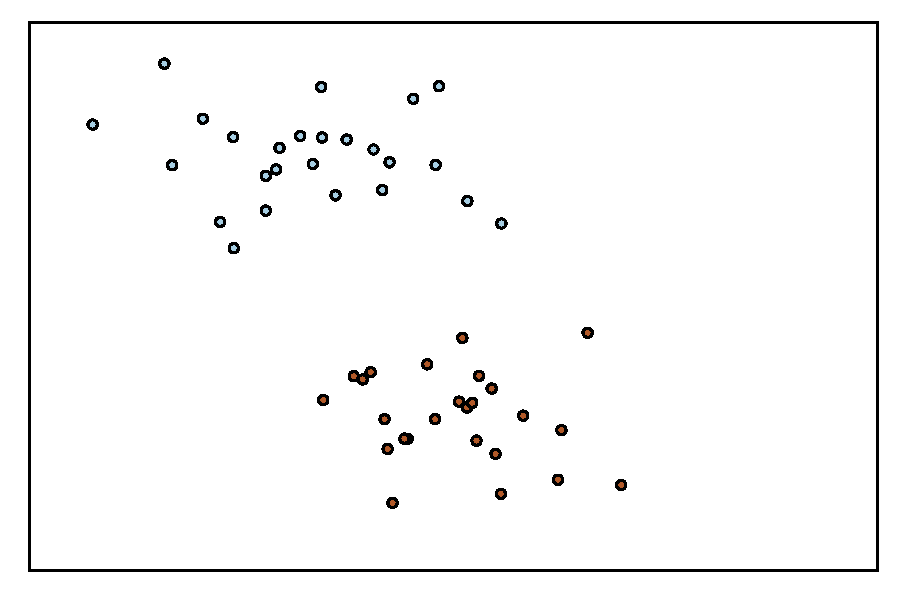
\includegraphics[width=0.6\textwidth]{Chapter2/SeparableProblem/separable_problem.pdf}
    \caption{Example of a binary classification problem, where classes are represented with colors blue and red, that is linearly separable.}
    \label{fig:separable_problem}
\end{figure}
Before illustrating the idea that leads to the \acrshort{svm} case, we have to define some concepts. Consider the sample of a binary classification problem:
\begin{equation}
    \nonumber
    \sample = \set{(x_i, y_i) \in \Xspace \times \Yspace, \; i=1, \ldots, \nsamples}
\end{equation}
where we typically use the class labels $\Yspace = \set{0, 1}$ or $\Yspace={-1, 1}$, and $\Xspace$ is usually $\reals^\dimx$. As we have seen, the goal in this problem is to find a rule $f: \Xspace \to \Yspace$ that minimizes the number of errors, namely $\emprisk(f) = \abs{\set{i: f(x_i) \neq y_i}}$, which using the labels $\Yspace = \set{0, 1}$ can be expressed as
\begin{equation}
    \nonumber
    \emprisk(f) = \sum_{i=1}^\nsamples (y_i - f(x_i))^2 .
\end{equation}
If, for a classification problem with sample $\sample$, there exists a rule $f(\cdot)$ such that all the instances are correctly classified, that is, its corresponding $\emprisk(f) = 0$, we say that the problem is separable; if this rule is linear, $f(x) = \dotp{w}{x} + b$, we say that the problem is linearly separable. That is, we can find a hyperplane that divides the space in two halves, and the two classes are completely contained in one of the halves, each in a different one. See Figure~\ref{fig:separable_problem} to see an example of such problems.
On the other hand, if for any linear rule $f$, its associated $\emprisk(f) > 0$, we say that the problem is not linearly separable. 
%
\begin{figure}[t!]
    \centering
    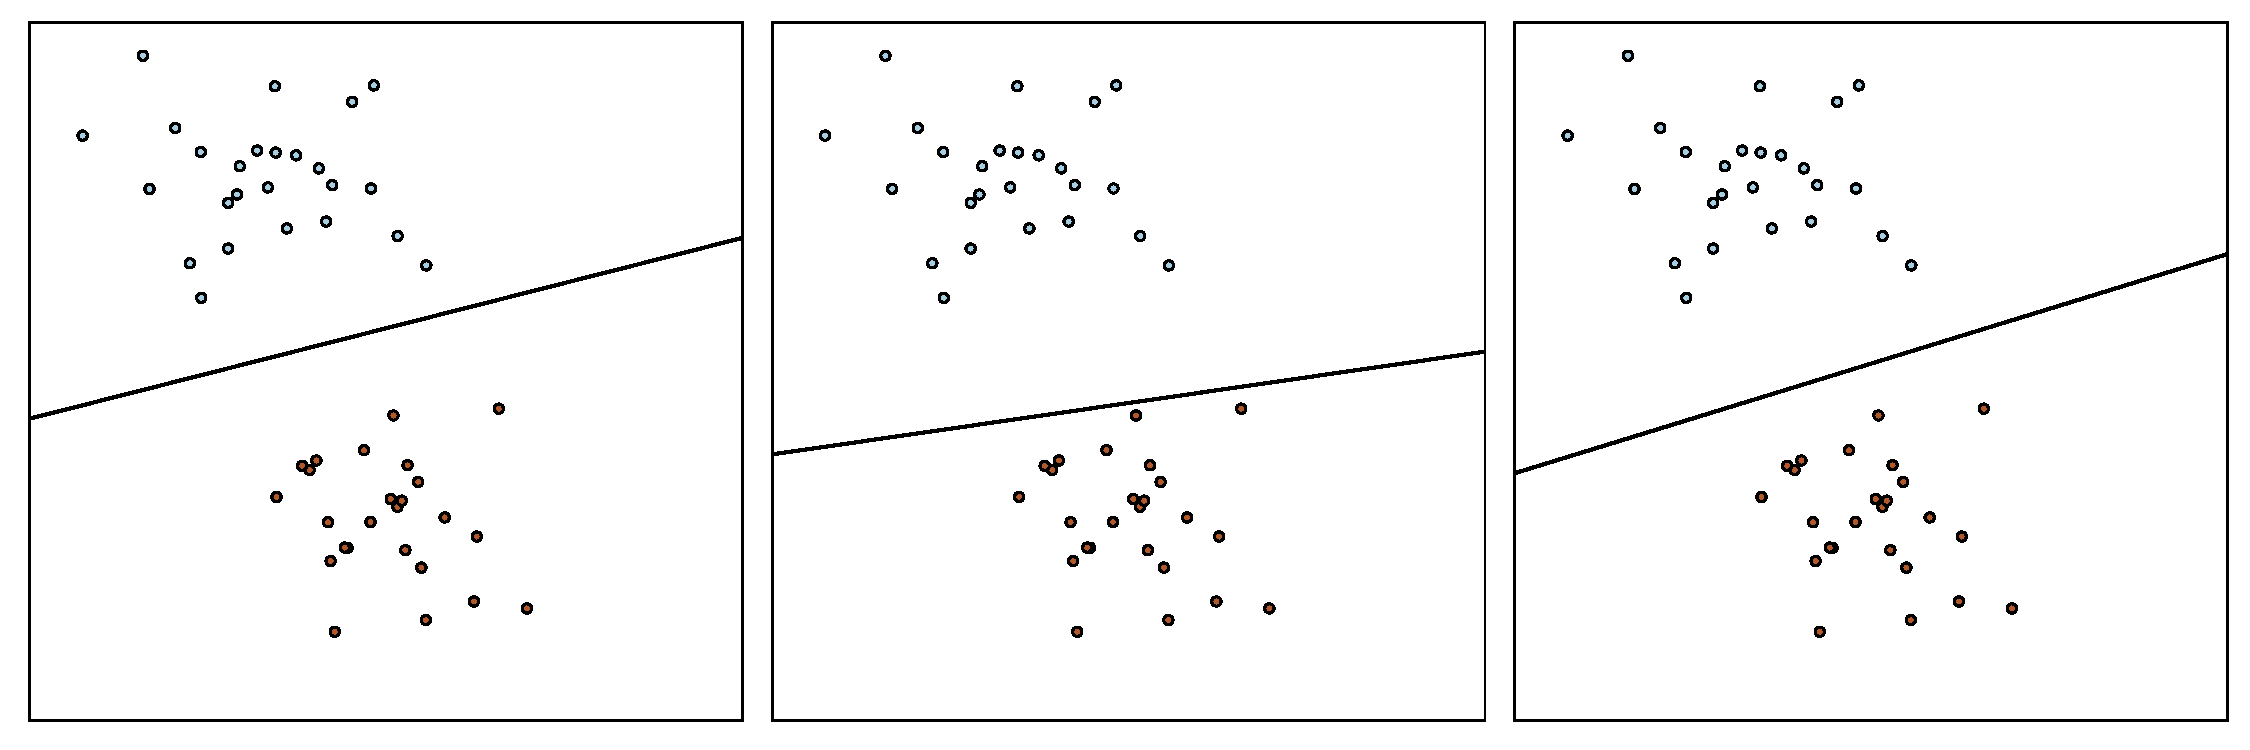
\includegraphics[width=\textwidth]{Chapter2/SeparableProblem/stochastic_boundaries.pdf}
    \caption{Separable problem with three different perfect classification rules.}
    \label{fig:stochastic_boundaries}
\end{figure}

Given a linearly separable problem, there might exist infinitely many linear functions that separate the two classes perfectly. See for example the previous example with three different boundaries that achieve perfect classification in Figure~\ref{fig:stochastic_boundaries}.
We may wonder then which is the best boundary among all those whose error is zero. Vapnik proposes to use maximum margin hyperplanes, that is, consider only those hyperplanes whose distance to the closest point is maximal.
Vapnik also shows that this kind of functions have better generalization properties, which have to do with the capacity of the hypothesis space.
%
The capacity of a set of functions is not easily interpretable, however, we can illustrate the properties of the maximum margin hyperplanes with the following reasoning. Given an empirical, training sample, we can learn a function that perfectly separate the two classes, but the corresponding boundary is very close to the points of one of the classes, say the red one in our example. If we sampled new points, we do not know if the boundary still achieve perfect classification, but it seems probable that some red points fall in the wrong side. See the middle example in Figure~\ref{fig:stochastic_boundaries} to illustrate this explanation.
%
However, if we select the boundary that is the furthest away from its closest points, we expect that such maximum margin boundary will be valid for new samples.
%
\begin{figure}[t!]
    \centering
    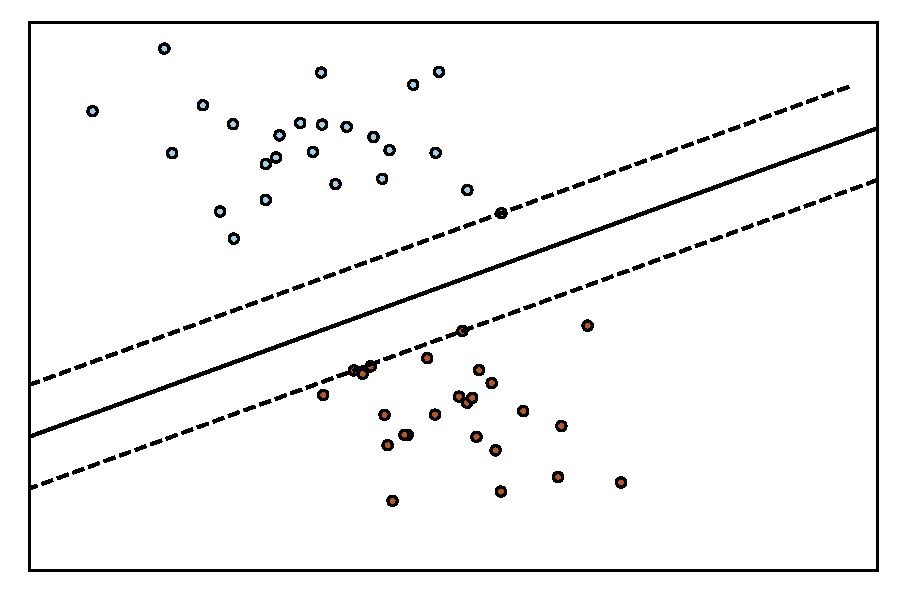
\includegraphics[width=0.6\textwidth]{Chapter2/SeparableProblem/maxmargin_boundary.pdf}
    \caption{Linearly separable problem separated by a maximum margin boundary. The classification boundary is shown with a solid line. The lines parallel to the boundary that contain the closest points to such boundary are depicted with dashed lines.}
    \label{fig:maxmargin_boundary}
\end{figure}
%
See in Fig our separable problem divided by a maximum margin hyperplane, which is a line in the two-dimensional case. We can see that in this case, the points from the sample are the furthest away possible from the boundary, which accounts for a better generalization to new data.

To find the maximum margin hyperplane, recall first the signed distance from a point $\tilde{x}$ to plane defined by $\dotp{w}{\cdot} + \hat{b} = 0$ is given by 
\begin{equation}
    \nonumber
    d(\tilde{x}) = \frac{1}{\norm{w}} (\dotp{w}{\tilde{x}} + b) ,
\end{equation}
where we replace $\frac{1}{\norm{w}} \hat{b}$ by the bias $b$.
Also, if we label the two classes using $\Yspace = \set{-1, 1}$, we can say that an instance $(x_i, y_i)$ is correctly classified when $$y_i \frac{1}{\norm{w}} \left(\dotp{w}{x_i} + b \right) > 0 .$$
Then, if we want to find that hyperplane that maximizes the margin while classifying all problems correctly, we can express it as
\begin{equation}\nonumber
    \begin{aligned}
        &\max_{w, b} & & m \\
        & \text{s.t.} & & y_i \frac{1}{\norm{w}} (\dotp{w}{\tilde{x}} + b) \geq m .         
    \end{aligned}  
\end{equation}
This is equivalent to the following problem 
\begin{equation}\nonumber
    \begin{aligned}
        &\max_{w, b} & & m \\
        & \text{s.t.} & & y_i (\dotp{w}{\tilde{x}} + b) \geq m \norm{w} ,       
    \end{aligned}  
\end{equation}
and, since the norm of the vector $w$ is not relevant, we can choose it such that $\norm{w} = 1 / m$; thus, the problem is given by
\begin{equation}\nonumber
    \begin{aligned}
        &\max_{w, b} & & \frac{1}{\norm{w}} \\
        & \text{s.t.} & & y_i (\dotp{w}{\tilde{x}} + b) \geq 1 ,       
    \end{aligned}  
\end{equation}
which has the same solutions as the following problem with easier derivatives:
\begin{equation}
    \label{eq:separable_primal}
    \begin{aligned}
        &\min_{w, b} & & \frac{1}{2} \norm{w}^2 \\
        & \text{s.t.} & & y_i (\dotp{w}{\tilde{x}} + b) \geq 1 .       
    \end{aligned}  
\end{equation}
%
Observe that in order to satisfy the constraints, it is not enough for the instances $(x_i, y_i)$ to be well classified, namely 
$$ y_i (\dotp{w}{\tilde{x}} + b) > 0 ,$$
but we are imposing a margin between the decision boundary and the data points, so the constraints are actually 
$$ y_i (\dotp{w}{\tilde{x}} + b) \geq 1 .$$
Therefore, we have expressed the problem of finding the maximum margin hyperplane as an optimization problem, like those that we have studied before in this chapter. However, this is an approach that is only valid for separable problems, however when using real-world data it is uncommon to find this kind of problems. To solve this issue, we have to introduce variables in the optimization problem that allow for misclassified points.

\subsection{Linear Support Vector Machines}
%
When we face a problem that is not linearly separable, it means that, for any rule $f(\cdot) = \dotp{w}{\cdot} + b$ there exist instances such that 
$$ y_j (\dotp{w}{x_j} + b) \leq 0 .$$
Moreover, when considering the constraints of the \acrshort{svm}, which wants to keep a margin, any instance $(x_j, y_j)$ such that 
$$ y_j (\dotp{w}{x_j} + b) < 1 $$
is not satisfying the constraints.
%
We can fix this by adding some slack variables $\xi_j \geq 0$ which we use to compensate in these contraints as
$$ y_i (\dotp{w}{x_i} + b) \geq 1 - \xi_i. $$
Now, for instances $(x_i, y_i)$ such that $y_i (\dotp{w}{x_i} + b) \geq 1$, its corresponding slack variable is $\xi_i = 0$. However, for instances such that $y_i (\dotp{w}{x_i} + b) < 1$, its corresponding slack variable is $\xi_i = 1 - y_i (\dotp{w}{x_i} + b)$, thus, $y_i (\dotp{w}{x_i} + b) = 1 - \xi_i .$
Summing it up, we can express then the slack variables as 
\begin{equation}
    \nonumber
    \xi_i = \pospart{1 - y_i (\dotp{w}{x_i} + b)} = \max(0, 1 - y_i (\dotp{w}{x_i} + b)),
\end{equation} 
which is the hinge loss function defined~\eqref{eq:hinge_def}, so the slack variables are also named hinge variables. 
Now we can give the definition of the optimization problem that corresponds to finding a maximum margin hyperplane with slack variables.
\begin{definition}[Primal Problem of \acrshort{svm} for Classification]
    Given a binary classification sample
    $$ \sample = \set{(x_i, l_i), \; i=1, \ldots, m} ,$$
    where $x_i \in \reals^\dimx$ are the feature vectors and $l_i \in \set{-1, 1}$ are the class labels, 
    the primal problem of the \acrshort{svm} for binary classification is:
    \begin{equation}
        \label{eq:linear_primal_clas}
        \begin{aligned}
            &\min_{w, b, \fv{\xi}} & & C \sum_{i=1}^m \xi_i + \frac{1}{2} \norm{w}^2 \\
            & \text{s.t.} & & l_i (\dotp{w}{x_i} + b) \geq 1 - \xi_i , \\
            & & & \xi_i \geq 0 ,      
        \end{aligned}  
    \end{equation}
    where $\fv{\xi} = (\xi_1, \ldots, \xi_m)^\intercal$, and $w, b, \fv{\xi}$ are the primal variables.
\end{definition}
Observe that this primal problem can be interpreted then as a regularized risk functional, where we have the risk term, where we use the hinge loss, and the regularization, penalizing $\norm{w}$; and where $C$ is a hyperparameter that regulates the trade-off between the margin and errors that the model commits.

% Regression
In the regression setting we need to define the primal problem differently. We again want to define a regularized risk functional, but we need to use a loss suited for regression. In the \acrshort{svm} for regression, the goal is to find a regression function such that the points are at a distance smaller than a given $\epsilon$. 
%
That is, given a training sample 
$$ \sample = \set{(x_i, t_i), i=1, \ldots, m}, $$
with $t_i \in \reals$ being the target values, the hard constraints to express this would be 
\begin{equation}
    \nonumber
    \abs{t_i - (\dotp{w}{x_i} + b) } \leq \epsilon,
\end{equation}
However, it is possible that there does not exist such function, so we introduce slack variables $\xi_i \geq 0$ again as
\begin{equation}
    \nonumber
    \abs{t_i - (\dotp{w}{x_i} + b) } \leq \epsilon + \xi_i,
\end{equation}
That is, the slack variables are defined as 
\begin{equation}
    \xi_i = \abs{t_i - (\dotp{w}{x_i} + b)}_\epsilon .
\end{equation}
That is, it is equivalent to using the $\epsilon$-insenstitive loss presented in~\eqref{eq:epsins_def}.
Getting rid of the absolute value, these constraints can be decomposed as
\begin{equation}
    \nonumber
   \dotp{w}{x_i} + b \geq t_i - \epsilon - \xi_i , \; \dotp{w}{x_i} + b \leq t_i + \epsilon + \hat{\xi}_i.
\end{equation}
Observe here that $$ \xi_i + \hat{\xi}_i = \abs{\dotp{\opt{w}}{x_i} + \opt{b} - t_i}_\epsilon ,$$
such that
\begin{itemize}
    \item $\xi_i = 0, \hat{\xi}_i = 0$: these are points inside the tube.
    \item $\xi_i = 0, \hat{\xi}_i > 0$: these are points above the tube.
    \item $\xi_i > 0, \hat{\xi}_i = 0$: these are points below the tube.
    \item $\xi_i > 0, \hat{\xi}_i > 0$: this is an impossible situation, since at any time a point satisfies one of the two constraints.
\end{itemize}
Therefore, we can also assert that $\xi_i \hat{\xi}_i = 0$.

Now, we can write the regression \acrshort{svm} primal problem
\begin{definition}[Primal Problem of \acrshort{svm} for Regression]
    Given a binary classification sample
    $$ \sample = \set{(x_i, t_i), \; i=1, \ldots, m} ,$$
    where $x_i \in \reals^\dimx$ are the feature vectors and $t_i \in \reals$ are the class labels, 
    the primal problem of the \acrshort{svm} for regression is:
    \begin{equation}
        \label{eq:linear_primal_reg}
        \begin{aligned}
            &\min_{w, b, \fv{\xi}} & & C \sum_{i=1}^m \left(\xi_i + \hat{\xi}_i\right) + \frac{1}{2} \norm{w}^2 \\
            & \text{s.t.} & & \dotp{w}{x_i} + b \geq t_i - \epsilon - \xi_i  , \\
            & & & \dotp{w}{x_i} + b \leq t_i + \epsilon + \hat{\xi}_i , \\
            & & & \xi_i \geq 0 , \hat{\xi}_i \geq 0 ,      
        \end{aligned}  
    \end{equation}
    where $\fv{\xi} = (\xi_1, \ldots, \xi_m)^\intercal$, and $w, b, \fv{\xi}$ are the primal variables.
\end{definition}
We have again defined then a regularized risk functional, where now the selected loss is the $\epsilon$-insensitive one. Again $C$ is the trade-off hyperparameter, but in this case we also have $\epsilon$ as the hyperparameter that defines the width of the tube insensitive to errors.

% Unifying formulation
In both cases, classification and regression we have defined corresponding optimization problems, which can be also interpreted as regularized risk functionals, that present some similarities. In fact, it is possible to express both problems using a unifying formulation, as we show next.
\begin{lemma}[Unifying Formulation for \acrshort{svm}]
    Given a sample
    $$ \sample = \set{(x_i, p_i), \; i=1, \ldots, \nsamples} ,$$
    where $x_i \in \reals^\dimx$ are the feature vectors and $p_i \in \reals$, 
    the primal problem defined as
    \begin{equation}
        \nonumber
        \begin{aligned}
            &\min_{w, b, \fv{\xi}} & & C \sum_{i=1}^\nsamples \xi_i + \frac{1}{2} \norm{w}^2 \\
            & \text{s.t.} & & y_i (\dotp{w}{x_i} + b) \geq p_i - \xi_i , \\
            & & & \xi_i \geq 0 ,      
        \end{aligned}  
    \end{equation}
    can be interpreted as the classification primal \acrshort{svm} problem~\eqref{eq:linear_primal_clas} when $\nsamples=m$ and
    $$ p_i = 1,\; y_i = l_i \text{ for } i=1, \ldots, m ;$$
    and can be interpreted as the regression primal \acrshort{svm} problem~\eqref{eq:linear_primal_reg} when $\nsamples = 2 m$ and
    \begin{equation}
        \nonumber
        \begin{aligned}
            & p_i = t_i - \epsilon ,\; &y_i &= 1 &\text{ for } i=1, \ldots, m ; \\
            & p_i = -t_i - \epsilon ,\; &y_i &= -1 &\text{ for } i=m+1, \ldots, 2m .
        \end{aligned}
    \end{equation}
\end{lemma}
%
\begin{definition}[Primal Problem - Unifying Formulation]
    Given a sample
    $$ \sample = \set{(x_i, p_i), \; i=1, \ldots, \nsamples} ,$$
    where $x_i \in \reals^\dimx$ are the feature vectors and $p_i \in \reals$, 
    we define the unified primal problem of \acrshort{svm} as
    \begin{equation}
        \label{eq:linear_primal}
        \begin{aligned}
            &\min_{w, b, \fv{\xi}} & & C \sum_{i=1}^\nsamples \xi_i + \frac{1}{2} \norm{w}^2 \\
            & \text{s.t.} & & y_i (\dotp{w}{x_i} + b) \geq p_i - \xi_i , \\
            & & & \xi_i \geq 0 ,      
        \end{aligned}  
    \end{equation}
    where $\fv{\xi} = (\xi_1, \ldots, \xi_\nsamples)^\intercal$, and $w, b, \fv{\xi}$ are the primal variables. Also, $C > 0$ is the trade-off hyperparameter.
\end{definition}
%
For the rest of this work we will use this formulation whenever it is not necessary to make a specific comment regarding the specific classification or regression characteristics.

\subsection{Solution and Analysis}
%
The problem defined in~\eqref{eq:linear_primal} is an optimization primal problem with a convex and differentiable objective function, and with affine constraint functions; then, we know from the strong duality theorem, presented in~\ref{th:strong_duality}, that we can use its corresponding dual problem to find the solution. Recall that to obtain the dual problem, defined in~\ref{def:dual_problem}, we need the Lagrangian function. In this case, the Lagrangian corresponding to~\ref{eq:linear_primal} is 
\begin{equation}
    \label{eq:linear_lagr}
    \lagr(w, b, \fv{\xi}, \fv{\alpha}, \fv{\beta}) = C \sum_{i=1}^\nsamples \xi_i + \frac{1}{2} \norm{w}^2 - \sum_{i=1}^\nsamples \alpha_i \left[ y_i (\dotp{w}{x_i} + b) - p_i + \xi_i \right] - \sum_{i=1}^\nsamples \beta_i \xi_i ,
\end{equation}
%
where $\fv{\alpha}, \fv{\beta} \geq 0$ are the Lagrange multipliers. Although in the general optimization problem explanations we used $\fv{\beta}$ for equality constraints, here we use it to discriminate between the two kinds of constraints in~\eqref{eq:linear_primal}. 
%
Now, the dual problem is defined as 
$$ \Theta(\fv{\alpha}, \fv{\beta}) = \inf_{w, b, \fv{\xi}} \lagr(w, b, \fv{\xi}, \fv{\alpha}, \fv{\beta}) . $$
Observe that $\lagr(w, b, \fv{\alpha}, \fv{\beta})$ is convex in all the primal variables, $w, b$ and $\fv{\xi}$, because the objective function is convex and the constraints are affine. Moreover, it is also differentiable in the primal variables, so to find the minimum of the Lagrangian in the primal variables is sufficient to take derivatives and select those points where these derivatives are zero:
\begin{align}
    \nabla_w \lagr(w, b, \fv{\xi}, \fv{\alpha}, \fv{\beta}) = 0 &\implies w = \sum_{i=1}^\nsamples y_i \alpha_i x_i , \label{eq:lagr_diff_w} \\
    \nabla_b \lagr(w, b, \fv{\xi}, \fv{\alpha}, \fv{\beta}) = 0 &\implies \sum_{i=1}^\nsamples y_i \alpha_i = 0, \label{eq:lagr_diff_b} \\
    \nabla_{\xi_i} \lagr(w, b, \fv{\xi}, \fv{\alpha}, \fv{\beta}) = 0 &\implies C - \alpha_i - \beta_i = 0 , \label{eq:lagr_diff_xi}
\end{align}
If we apply these results in the Lagrangian, we get a simpler formula. Using~\eqref{eq:lagr_diff_b} the terms with $b$ disappear, and with~\eqref{eq:lagr_diff_xi} all the terms with $\xi_i$ vanish as well. Then, substiuting $w$ according to~\eqref{eq:lagr_diff_w}, we get 
\begin{equation}
    \nonumber
    \begin{aligned}
        \inf_{w, b, \fv{\xi}} \lagr(w, b, \fv{\xi}, \fv{\alpha}, \fv{\beta}) &= \frac{1}{2} \dotp{\sum_{i=1}^\nsamples y_i \alpha_i x_i}{\sum_{i=1}^\nsamples y_i \alpha_i x_i} \\
        &\quad- \sum_{i=1}^\nsamples \alpha_i \left[y_i \dotp{\sum_{j=1}^\nsamples y_j \alpha_j x_j}{x_i}  \right] + \sum_{i=1}^\nsamples \alpha_i p_i \\
        &= -\frac{1}{2} \sum_{i=1}^\nsamples \sum_{j=1}^\nsamples y_i y_j \alpha_i \alpha_j \dotp{x_i}{x_j} + \sum_{i=1}^\nsamples \alpha_i p_i .
    \end{aligned}
\end{equation}
We observe here that $\fv{\beta}$ disappear from the dual objective function $\Theta$. However, we still have to take into account that we have used~\eqref{eq:lagr_diff_b} and~\eqref{eq:lagr_diff_xi}. From~\eqref{eq:lagr_diff_xi}, since $\beta_i \geq 0$, we get that $\alpha_i \leq C$. Then, the dual problem can be defined as follows.
\begin{definition}[Dual Problem - Unifying Formulation]
    The dual problem corresponding to problem~\eqref{eq:linear_primal} is
    \begin{equation}
        \label{eq:linear_dual}
        \begin{aligned}
            &\min_{\fv{\alpha}} & & \frac{1}{2} \sum_{i=1}^\nsamples \sum_{j=1}^\nsamples y_i y_j \alpha_i \alpha_j \dotp{x_i}{x_j} - \sum_{i=1}^\nsamples \alpha_i p_i \\
            & \text{s.t.} & & \sum_{i=1}^\nsamples y_i \alpha_i = 0 , \\
            & & & 0 \leq \alpha_i \leq C ,      
        \end{aligned}  
    \end{equation}
    where the first constraint is named equality constraint and the rest are the box constraints.
\end{definition}
The result is a constrained quadratic problem where the first term is quadratic and the second is linear. Algorithms, like the \acrfull{smo}~\citep{KeerthiSBM01}, have been developed to solve this dual problem efficiently. Moreover, optimized implementations of \acrshort{smo} are available, like the one in \texttt{LIBSVM}~\citep{ChangL11}.

%
Observe that~\eqref{eq:linear_dual} is a convex problem, so it has a single value $\opt{\fv{\alpha}}$ that is a solution. Therefore, by solving the dual problem, using algorithms like \acrshort{smo}, we obtain this optimal $\opt{\fv{\alpha}}$; then, using~\eqref{eq:lagr_diff_w} we can recover the optimal primal variable $\opt{w}$ as 
\begin{equation}
    \nonumber
    \opt{w} = \sum_{i=1}^\nsamples y_i \opt{\alpha}_i x_i .
\end{equation}
%
Observe that the primal problem~\eqref{eq:linear_primal} has convex, differentiable objective function and affine constraints, which satisfy the conditions from Theorem~\ref{th:kkt_conditions}; thus, the \acrshort{kkt} conditions are necessary.
%
Concretely, the complementary slackness condition~\eqref{eq:kkt_comp} in our case can be expressed as
\begin{align}
    \opt{\alpha}_i \left[ y_i (\dotp{\opt{w}}{x_i} + \opt{b}) - p_i + \opt{\xi}_i \right] = 0 , \label{eq:comp_alpha} \\
    \opt{\beta}_i \opt{\xi}_i = 0 , \label{eq:comp_beta}
\end{align}
for all $i=1, \ldots, \nsamples$. 
Now we realize from~\eqref{eq:comp_alpha} that when $y_i (\dotp{\opt{w}}{x_i} + \opt{b}) - p_i + \opt{\xi}_i > 0$, the corresponding dual variable must be $\alpha_i = 0$. Therefore, the primal solution $\opt{w}$ is 
\begin{equation}
    \nonumber
    \opt{w} = \sum_{i \in \svset} y_i \opt{\alpha}_i x_i ,
\end{equation}
where the elements of the set $\set{i: \alpha_i = 0}$ or $\svset = \set{i: y_i (\dotp{\opt{w}}{x_i} + \opt{b}) - p_i + \opt{\xi}_i = 0}$ receive the name of support vectors.
%

We still have to see how we can recover the other primal variables $\opt{\fv{\xi}}$ and $\opt{b}$. For this goal, the \acrshort{kkt} conditions will be useful.
Recall that $\alpha_i$ and $\beta_i$ are connected through~\eqref{eq:lagr_diff_xi}, such that 
$$ \opt{\alpha}_i + \opt{\beta}_i = C .$$
Therefore, when $0 < \alpha_i < C$, and, thus, $\beta_i \neq 0$, we have from~\eqref{eq:comp_beta} that $\opt{\xi}_i = 0$ and, in consequence from~\eqref{eq:comp_alpha},
\begin{equation}
    \nonumber
    y_i (\dotp{\opt{w}}{x_i} + \opt{b}) - p_i = 0 .
\end{equation}
That is, we can recover $\opt{b}$ from the set of indices $\set{i: 0 < \alpha_i < C}$.
%
After obtaining $\opt{b}$, we focus on the indices $i$ such that $\opt{\alpha}_i = C$, so $\opt{\beta}_i = 0$ and, since~\eqref{eq:comp_beta} is satisfied, $\opt{\xi}_i$ is not necessarily $0$. Then, we can apply~\eqref{eq:comp_alpha} to get the solutions $\opt{\xi}_i$ from 
\begin{equation}
    \nonumber
    y_i (\dotp{\opt{w}}{x_i} + \opt{b}) - p_i - \opt{\xi}_i = 0 .
\end{equation}

%
Actually, we can sum this up and use these necessary \acrshort{kkt} conditions, equations~\eqref{eq:comp_alpha} and~\eqref{eq:comp_beta}, to establish a classification of the support vectors according to its corresponding $\opt{\alpha}_i$, which we give in Table~\ref{tab:sv_clas}.
%
\begin{table}[t!]
    \caption{Classification of the support vectors in terms of the value of $\opt{\alpha}_i$.}
    \label{tab:sv_clas}
    \centering
    \scalebox{1}{
     \begin{tabular}{*{4}{c}}
     \toprule
     \fhead{$\opt{\alpha}_i$} & \fhead{$\opt{\beta}_i$} & \fhead{$\opt{\xi}_i$} & \fhead{$y_i (\dotp{\opt{w}}{x_i} + \opt{b})$}   \\
     \midrule
     $0 < \opt{\alpha}_i < C$ & $\opt{\beta} > 0$ & $\opt{\xi}_i = 0$ & $y_i (\dotp{\opt{w}}{x_i} + \opt{b}) = p_i$ \\
     $\opt{\alpha}_i = C$ & $\opt{\beta} = 0$ & $0 < \opt{\xi}_i < p_i$ & $0 < y_i (\dotp{\opt{w}}{x_i} + \opt{b}) < p_i$ \\
     $\opt{\alpha}_i = C$ & $\opt{\beta} = 0$ & $p_i \leq \opt{\xi}_i $ & $y_i (\dotp{\opt{w}}{x_i} + \opt{b}) \leq 0$ \\
      \bottomrule
     \end{tabular}
     }
\end{table}
%
To study the meaning of this table, we will consider first the binary classification setting, where $y_i = l_i$ and $p_i=1$ for all $i=1, \ldots, \nsamples$. The first row correspond to points where $l_i (\dotp{\opt{w}}{x_i} + \opt{b}) = 1$, that is, points that are correctly classified and are just on the margin. The points from the second row are also points that are correctly classified, but they lie inside the margin. Finally, the points in the third row are misclassified.
Therefore, the predictions of the \acrshort{svm} in the classification settings depend only on those points that lie over the margin, inside the margin, or are misclassified. The points that are correctly classified but outside the margin do not play any role in the final model.
%

In the case of regression, we need to observe again that 
$$ \xi_i + \hat{\xi}_i = \xi_i + {\xi}_{\nsamples + i} = \abs{\dotp{\opt{w}}{x_i} + \opt{b} - t_i}_\epsilon ,$$
and $\xi_i {\xi}_{\nsamples + i} = 0$ 
% Consider first the case where $y_i = 1$ and $p_i = t_i - \epsilon$.
Consider the first row, if $\xi_i = 0$, as in the first row, then $\dotp{\opt{w}}{x_i} + \opt{b} = t_i - \epsilon$ is  a point in the lower border of the $\epsilon$-tube. If $\xi_{i + \nsamples} = 0$, as in the first row, then $\dotp{\opt{w}}{x_i} + \opt{b} = t_i + \epsilon$ is  a point in the upper border of the $\epsilon$-tube.
%
In the second and third rows, if $\xi_i > 0$, then ${\xi}_{i + \nsamples} = 0$, and we have points such that $\dotp{\opt{w}}{x_i} + \opt{b} < t_i - \epsilon$, that is, below the tube. 
Analogously, if ${\xi}_{i + \nsamples} > 0$, we have points above the tube.
%
% In summary, the solutions of the \acrshort{svm} are composed only from ``extreme points'', those that are difficult to classify or are far from the regressor function.


\subsection{Kernel Extension}
Observe that the dual problem~\eqref{eq:linear_dual} depends only on the inner product between the feature vectors $x_i$. Also, observe that, using the result from~\eqref{eq:lagr_diff_w} we can write the prediction for a new instance $\tilde{x}$ as 
\begin{equation}
    \nonumber
    \dotp{\opt{w}}{\tilde{x}} + \opt{b} = \sum_{i = 1}^\nsamples y_i \opt{\alpha}_i \dotp{x_i}{\tilde{x}} + \opt{b} .
\end{equation} 
This result is similar to that of the representer theorem, presented in Theorem~\ref{th:repr_theorem}.
In fact, consider the following model 
$f(\cdot) = \dotp{w}{\phi(\cdot)} + b$
where we are using the transformation $\phi: \reals^\dimx \to \rkhs$ and $\rkhs$ is some \acrshort{rkhs} with reproducing kernel $k$, such that for all $x, \tilde{x} \in \reals^\dimx$, 
$$ \dotp{\phi(x)}{\phi(\tilde{x})} = k(x, \tilde{x}) .$$ 
Now, we are not looking for a maximum margin hyperplane in the original feature space $\reals^\dimx$, but in a possibly infinite-dimensional space $\rkhs$.
The primal problem for the kernel extension using the unified formulation is
\begin{equation}
    \label{eq:kernel_primal}
    \begin{aligned}
        &\min_{w, b, \fv{\xi}} & & C \sum_{i=1}^\nsamples \xi_i + \frac{1}{2} \norm{w}^2 \\
        & \text{s.t.} & & y_i (\dotp{w}{\phi(x_i)} + b) \geq p_i - \xi_i , \\
        & & & \xi_i \geq 0 ,      
    \end{aligned}  
\end{equation}
Its corresponding Lagrangian is then 
\begin{equation}
    \nonumber
    %\label{eq:kernel_lagr}
    \lagr(w, b, \fv{\xi}, \fv{\alpha}, \fv{\beta}) = \sum_{i=1}^\nsamples \xi_i + \frac{1}{2} \norm{w}^2 - \sum_{i=1}^\nsamples \alpha_i \left[ y_i (\dotp{w}{\phi(x_i)} + b) - p_i + \xi_i \right] - \sum_{i=1}^\nsamples \beta_i \xi_i ,
\end{equation}
and the optimal value for the variable $w$, which in the linear case was given in~\ref{eq:lagr_diff_w}, is now
\begin{equation}\label{eq:lagr_diff_w_kernel}
    \nabla_w \lagr(w, b, \fv{\xi}, \fv{\alpha}, \fv{\beta}) = 0 \implies w = \sum_{i=1}^\nsamples y_i \alpha_i \phi(x_i) .
\end{equation}
Recall that in the case of infinite-dimensional case, we have that $\phi(x_i)$ are real-valued functions with domain in $\reals^\dimx$, and so is $\opt{w}$ then, that is 
$\opt{w}: \reals^\dimx \to \reals$. 
Since $k$ is a reproducing kernel, we can also express this as 
\begin{equation}
    \nonumber
    \opt{w}(\cdot) = \dotp{\opt{w}}{\phi(\cdot)} = \sum_{i=1}^\nsamples y_i \opt{\alpha}_i k(x_i, \cdot),
\end{equation}
as the Representer Theorem indicates for a regularized risk functional like~\eqref{eq:kernel_primal}.
%
Repeating the procedure that we have shown for the linear case, we can obtain the corresponding dual problem, which is the following.
\begin{equation}
    \label{eq:kernel_dual}
    \begin{aligned}
        &\min_{\fv{\alpha}} & & \frac{1}{2} \sum_{i=1}^\nsamples \sum_{j=1}^\nsamples y_i y_j \alpha_i \alpha_j k(x_i, x_j) - \sum_{i=1}^\nsamples \alpha_i p_i \\
        & \text{s.t.} & & \sum_{i=1}^\nsamples y_i \alpha_i = 0 , \\
        & & & 0 \leq \alpha_i \leq C ,      
    \end{aligned}  
\end{equation}
where we use that $k(x_i, x_j) = \dotp{\phi(x_i)}{\phi(x_j)}$.
%
We can express both the dual problem using a matrix formulation as 
\begin{equation}
    \label{eq:kernel_dual_matrix}
    \begin{aligned}
        &\min_{\fv{\alpha}} & & \frac{1}{2} \fv{\alpha}^\intercal \fm{Q} \fv{\alpha} - \fv{\alpha}^\intercal \fv{p} \\
        & \text{s.t.} & & \sum_{i=1}^\nsamples y_i \alpha_i = 0 , \\
        & & & 0 \leq \alpha_i \leq C ,      
    \end{aligned}  
\end{equation}
with $\fv{p} = (p_1, \ldots, p_\nsamples)^\intercal$. Here, $Q$ is called the kernel matrix and is defined as 
$$ Q_{ij} = y_i y_j k(x_i, x_j) $$
in the case of the kernelized case, or as 
$$ Q_{ij} = y_i y_j \dotp{x_i}{x_j} $$
in the linear one.

%\subsection{Connection with Structural Learning}
\subsection{SVM Variants}
The \acrshort{svm} has experienced a great popularity for many years, and several modifications and extensions have been proposed. In this work we will consider two relevant variants: the L2 and LS-\acrshort{svm}, and we can also refer to the standard \acrshort{svm} as L1-\acrshort{svm} to differentiate it from these variants.
%
For compactness, we will consider the non-linear models to present these variants, namely 
$$ f(\cdot) = \dotp{w}{\phi(\cdot)} + b ,$$
which can be reduced to the linear case just by selecting $\phi$ as the identity function.

\subsubsection*{L2-\acrshort{svm}}
The idea motivating the L2-\acrshort{svm}~\citep{Burges98} variant is replacing the loss functions used in the L1-\acrshort{svm} for their squared counterparts. 
The hinge loss, used for classification and defined in~\eqref{eq:hinge_def}, is replaced by the squared hinge loss, as defined as~\eqref{eq:sqhinge_def}.
The $\epsilon$-insensitive loss defined as~\eqref{eq:epsins_def}, which is used in the regression L1-\acrshort{svm}, is replaced by the squared-hinge loss as defined in~\eqref{eq:sqepsins_def}.
%

We can give then the definitions of the L2-\acrshort{svm} problems for classification and regression.
\begin{definition}[Primal Problem of L2-\acrshort{svm} for Classification]
    Given a binary classification sample
    $$ \sample = \set{(x_i, l_i), \; i=1, \ldots, m} ,$$
    where $x_i \in \reals^\dimx$ are the feature vectors and $l_i \in \set{-1, 1}$ are the class labels, 
    the primal problem of the L2-\acrshort{svm} for binary classification is:
    \begin{equation}
        \label{eq:l2_primal_clas}
        \begin{aligned}
            &\min_{w, b, \fv{\xi}} & & \frac{C}{2} \sum_{i=1}^m (\xi_i)^2 + \frac{1}{2} \norm{w}^2 \\
            & \text{s.t.} & & l_i (\dotp{w}{\phi(x_i)} + b) \geq 1 - \xi_i , 
        \end{aligned}  
    \end{equation}
    where $\fv{\xi} = (\xi_1, \ldots, \xi_m)^\intercal$, and $w, b, \fv{\xi}$ are the primal variables.
\end{definition}
%
\begin{definition}[Primal Problem of L2-\acrshort{svm} for Regression]
    Given a binary classification sample
    $$ \sample = \set{(x_i, t_i), \; i=1, \ldots, m} ,$$
    where $x_i \in \reals^\dimx$ are the feature vectors and $t_i \in \reals$ are the class labels, 
    the primal problem of the L2-\acrshort{svm} for regression is:
    \begin{equation}
        \label{eq:l2_primal_reg}
        \begin{aligned}
            &\min_{w, b, \fv{\xi}} & & \frac{C}{2} \sum_{i=1}^m \left((\xi_i)^2 + (\hat{\xi}_i)^2 \right) + \frac{1}{2} \norm{w}^2 \\
            & \text{s.t.} & & \dotp{w}{\phi(x_i)} + b \geq t_i - \epsilon - \xi_i  , \\
            & & & \dotp{w}{\phi(x_i)} + b \leq t_i + \epsilon + \hat{\xi}_i , 
        \end{aligned}  
    \end{equation}
    where $\fv{\xi} = (\xi_1, \ldots, \xi_m)^\intercal$, and $w, b, \fv{\xi}$ are the primal variables.
\end{definition}
%
Observe in both cases that, since the slack variables are squared in the objective function, the constraints to enforce that these slack variables are non-negative are no longer needed.
As with the L1-\acrshort{svm}, we will use a formulation to unify both problems and show a development that is valid for both cases. 
%
%
\begin{lemma}[Unifying Formulation for L2-\acrshort{svm}]
    Given a sample
    $$ \sample = \set{(x_i, p_i), \; i=1, \ldots, \nsamples} ,$$
    where $x_i \in \reals^\dimx$ are the feature vectors and $p_i \in \reals$, 
    the primal problem defined as
    \begin{equation}
        \nonumber
        \begin{aligned}
            &\min_{w, b, \fv{\xi}} & & \frac{C}{2} \sum_{i=1}^\nsamples (\xi_i)^2 + \frac{1}{2} \norm{w}^2 \\
            & \text{s.t.} & & y_i (\dotp{w}{x_i} + b) \geq p_i - \xi_i ,     
        \end{aligned}  
    \end{equation}
    can be interpreted as the classification primal L2-\acrshort{svm} problem~\eqref{eq:l2_primal_clas} when $\nsamples=m$ and
    $$ p_i = 1,\; y_i = l_i \text{ for } i=1, \ldots, m ;$$
    and can be interpreted as the regression primal L2-\acrshort{svm} problem~\eqref{eq:l2_primal_reg} when $\nsamples = 2 m$ and
    \begin{equation}
        \nonumber
        \begin{aligned}
            & p_i = t_i - \epsilon ,\; &y_i &= 1 &\text{ for } i=1, \ldots, m ; \\
            & p_i = -t_i - \epsilon ,\; &y_i &= -1 &\text{ for } i=m+1, \ldots, 2m .
        \end{aligned}
    \end{equation}
\end{lemma}
%
\begin{definition}[Primal Problem - Unifying Formulation for L2-\acrshort{svm}]
    Given a sample
    $$ \sample = \set{(x_i, p_i), \; i=1, \ldots, \nsamples} ,$$
    where $x_i \in \reals^\dimx$ are the feature vectors and $p_i \in \reals$, 
    we define the unified primal problem of L2-\acrshort{svm} as
    \begin{equation}
        \label{eq:l2_primal}
        \begin{aligned}
            &\min_{w, b, \fv{\xi}} & & \frac{C}{2} \sum_{i=1}^\nsamples \xi_i + \frac{1}{2} \norm{w}^2 \\
            & \text{s.t.} & & y_i (\dotp{w}{\phi(x_i)} + b) \geq p_i - \xi_i ,      
        \end{aligned}  
    \end{equation}
    where $\fv{\xi} = (\xi_1, \ldots, \xi_\nsamples)^\intercal$, and $w, b, \fv{\xi}$ are the primal variables. Also, $C > 0$ is the trade-off hyperparameter.
\end{definition}
%
We follow an analogous procedure to the one we have used for the standard \acrshort{svm}. The Lagrangian corresponding to the primal problem~\eqref{eq:l2_primal} is 
\begin{equation}
    \label{eq:l2_lagr}
    \lagr(w, b, \fv{\xi}, \fv{\alpha}) = \frac{C}{2} \sum_{i=1}^\nsamples (\xi_i)^2 + \frac{1}{2} \norm{w}^2 - \sum_{i=1}^\nsamples \alpha_i \left[ y_i (\dotp{w}{\phi(x_i)} + b) - p_i + \xi_i \right] ,
\end{equation}
%
where $\fv{\alpha} \geq 0$ are the Lagrange multipliers.
%
Again, the dual problem is defined as 
$$ \Theta(\fv{\alpha}) = \inf_{w, b, \fv{\xi}} \lagr(w, b, \fv{\xi}, \fv{\alpha}) , $$
and $\lagr(w, b, \fv{\alpha})$ is convex in all the primal variables, $w, b$ and $\fv{\xi}$. Therefore, to find the minimum of the Lagrangian in the primal variables is sufficient to take derivatives and make them zero:
\begin{align}
    \nabla_w \lagr(w, b, \fv{\xi}, \fv{\alpha}) = 0 &\implies w = \sum_{i=1}^\nsamples y_i \alpha_i \phi(x_i) , \label{eq:lagr_diff_w_l2} \\
    \nabla_b \lagr(w, b, \fv{\xi}, \fv{\alpha}) = 0 &\implies \sum_{i=1}^\nsamples y_i \alpha_i = 0, \label{eq:lagr_diff_b_l2} \\
    \nabla_{\xi_i} \lagr(w, b, \fv{\xi}, \fv{\alpha}) = 0 &\implies C \xi_i - \alpha_i  = 0 , \label{eq:lagr_diff_xi_l2}
\end{align}
If we apply these results in the Lagrangian, we get a simpler formula. Using~\eqref{eq:lagr_diff_b} the terms with $b$ disappear, and with~\eqref{eq:lagr_diff_xi} all the terms with $\xi_i$ vanish as well. Then, substiuting $w$ according to~\eqref{eq:lagr_diff_w}, we get 
\begin{equation}
    \nonumber
    \begin{aligned}
        \inf_{w, b, \fv{\xi}} \lagr(w, b, \fv{\xi}, \fv{\alpha}) &= \frac{1}{2C} \sum_{i=1}^\nsamples \alpha_i^2 + \frac{1}{2} \dotp{\sum_{i=1}^\nsamples y_i \alpha_i \phi(x_i)}{\sum_{i=1}^\nsamples y_i \alpha_i \phi(x_i)} \\
        &\quad- \sum_{i=1}^\nsamples \alpha_i \left[y_i \dotp{\sum_{j=1}^\nsamples y_j \alpha_j \phi(x_j)}{\phi(x_i)}  \right] - \frac{1}{C} \sum_{i=1}^\nsamples \alpha_i^2 + \sum_{i=1}^\nsamples \alpha_i p_i  \\
        &= -\frac{1}{2} \sum_{i=1}^\nsamples \sum_{j=1}^\nsamples y_i y_j \alpha_i \alpha_j \dotp{\phi(x_i)}{\phi(x_j)} - \frac{1}{2C} \sum_{i=1}^\nsamples \alpha_i^2 + \sum_{i=1}^\nsamples \alpha_i p_i .
    \end{aligned}
\end{equation}
We observe here that now the partial derivative with respect to $\xi$, given in~\eqref{eq:lagr_diff_xi_l2}, does not establish an upper bound for $\alpha_i$, but a new term with $\alpha_i^2$ appears in the dual objective function.
%
We can define now the L2-\acrshort{svm} dual problem.
\begin{definition}[Dual Problem - Unifying Formulation for L2-\acrshort{svm}]
    The dual problem corresponding to problem~\eqref{eq:linear_primal} is
    \begin{equation}
        \label{eq:l2_dual_matrix}
        \begin{aligned}
            &\min_{\fv{\alpha}} & & \frac{1}{2} \fv{\alpha}^\intercal \left( \fm{Q} + \frac{1}{C} \fm{I}_\nsamples \right)\fv{\alpha} - \fv{\alpha}^\intercal \fv{p} \\
            & \text{s.t.} & & \sum_{i=1}^\nsamples y_i \alpha_i = 0 , \\
            & & & \alpha_i \geq 0 .
        \end{aligned}  
    \end{equation}
\end{definition}
Observe that we again obtain a quadratic optimization problem, as in the L1-\acrshort{svm} case, where we do no longer have the box constraints, but we have a diagonal matrix that is added to the kernel matrix. That is, there is not an upper bound for $\alpha_i$, but the diagonal term can be interpreted as a soft constraint for the size of $\fv{\alpha}$. 


\subsubsection*{LS-\acrshort{svm}}
%
The LS-\acrshort{svm}~\citep{SuykensV99} replaces the losses of the L1-\acrshort{svm} for the squared loss.
Even in classification, where the aim is to regress to the values $1$ and $-1$ the positive and negative classes.
To do this, the inequality constraints are replaced by equality ones.
%
We give the definitions of the LS-\acrshort{svm} problems for classification and regression next.
\begin{definition}[Primal Problem of LS-\acrshort{svm} for Classification]
    Given a binary classification sample
    $$ \sample = \set{(x_i, l_i), \; i=1, \ldots, m} ,$$
    where $x_i \in \reals^\dimx$ are the feature vectors and $l_i \in \set{-1, 1}$ are the class labels, 
    the primal problem of the LS-\acrshort{svm} for binary classification is:
    \begin{equation}
        \label{eq:ls_primal_clas}
        \begin{aligned}
            &\min_{w, b, \fv{\xi}} & & \frac{C}{2} \sum_{i=1}^m (\xi_i)^2 + \frac{1}{2} \norm{w}^2 \\
            & \text{s.t.} & & l_i (\dotp{w}{\phi(x_i)} + b) = 1 - \xi_i , 
        \end{aligned}  
    \end{equation}
    where $\fv{\xi} = (\xi_1, \ldots, \xi_m)^\intercal$, and $w, b, \fv{\xi}$ are the primal variables.
\end{definition}
%
\begin{definition}[Primal Problem of LS-\acrshort{svm} for Regression]
    Given a binary classification sample
    $$ \sample = \set{(x_i, t_i), \; i=1, \ldots, m} ,$$
    where $x_i \in \reals^\dimx$ are the feature vectors and $t_i \in \reals$ are the class labels, 
    the primal problem of the LS-\acrshort{svm} for regression is:
    \begin{equation}
        \label{eq:ls_primal_reg}
        \begin{aligned}
            &\min_{w, b, \fv{\xi}} & & \frac{C}{2} \sum_{i=1}^m (\xi_i)^2 + \frac{1}{2} \norm{w}^2 \\
            & \text{s.t.} & & \dotp{w}{\phi(x_i)} + b = t_i - \xi_i  , \\
        \end{aligned}  
    \end{equation}
    where $\fv{\xi} = (\xi_1, \ldots, \xi_m)^\intercal$, and $w, b, \fv{\xi}$ are the primal variables.
\end{definition}
%
As with the other variants, we want to use a unifying formulation for the regression and classification problems.

\begin{lemma}[Unifying Formulation for LS-\acrshort{svm}]
    Given a sample
    $$ \sample = \set{(x_i, p_i), \; i=1, \ldots, \nsamples} ,$$
    where $x_i \in \reals^\dimx$ are the feature vectors and $p_i \in \reals$, 
    the primal problem defined as
    \begin{equation}
        \nonumber
        \begin{aligned}
            &\min_{w, b, \fv{\xi}} & & \frac{C}{2} \sum_{i=1}^\nsamples (\xi_i)^2 + \frac{1}{2} \norm{w}^2 \\
            & \text{s.t.} & & y_i (\dotp{w}{x_i} + b) = p_i - \xi_i ,     
        \end{aligned}  
    \end{equation}
    can be interpreted as the classification primal LS-\acrshort{svm} problem~\eqref{eq:ls_primal_clas} when $\nsamples=m$ and
    $$ p_i = 1,\; y_i = l_i \text{ for } i=1, \ldots, m ;$$
    and can be interpreted as the regression primal LS-\acrshort{svm} problem~\eqref{eq:ls_primal_reg} when $\nsamples = m$ and
    \begin{equation}
        \nonumber
        \begin{aligned}
            p_i = t_i  ,\; y_i = 1 \text{ for } i=1, \ldots, m ; \\
        \end{aligned}
    \end{equation}
\end{lemma}
%
\begin{definition}[Primal Problem - Unifying Formulation for LS-\acrshort{svm}]
    Given a sample
    $$ \sample = \set{(x_i, p_i), \; i=1, \ldots, \nsamples} ,$$
    where $x_i \in \reals^\dimx$ are the feature vectors and $p_i \in \reals$, 
    we define the unified primal problem of LS-\acrshort{svm} as
    \begin{equation}
        \label{eq:ls_primal}
        \begin{aligned}
            &\min_{w, b, \fv{\xi}} & & \frac{C}{2} \sum_{i=1}^\nsamples \xi_i + \frac{1}{2} \norm{w}^2 \\
            & \text{s.t.} & & y_i (\dotp{w}{\phi(x_i)} + b) = p_i - \xi_i ,      
        \end{aligned}  
    \end{equation}
    where $\fv{\xi} = (\xi_1, \ldots, \xi_\nsamples)^\intercal$, and $w, b, \fv{\xi}$ are the primal variables. Also, $C > 0$ is the trade-off hyperparameter.
\end{definition}
%
The corresponding Lagrangian to the primal problem~\eqref{eq:ls_primal} is 
\begin{equation}
    \label{eq:ls_lagr}
    \lagr(w, b, \fv{\xi}, \fv{\alpha}) = \frac{C}{2} \sum_{i=1}^\nsamples (\xi_i)^2 + \frac{1}{2} \norm{w}^2 - \sum_{i=1}^\nsamples \alpha_i \left[ y_i (\dotp{w}{\phi(x_i)} + b) - p_i + \xi_i \right] ,
\end{equation}
%
where $\fv{\alpha} \in \reals$ are the Lagrange multipliers. Observe that we do no longer need the non-negativity of these variables, because they correspond to equality instead of inequality constraints.
%
Now we use \acrshort{kkt} conditions to find the solutions to the optimization problem. Recall that the \acrshort{kkt} are sufficient conditions, and for problems with convex, differentiable objective function with affine constraints can be expressed as:
\begin{align}
    \nabla_w \lagr(w, b, \fv{\xi}, \fv{\alpha}) = 0 &\implies w = \sum_{i=1}^\nsamples y_i \alpha_i \phi(x_i) , \label{eq:lagr_diff_w_ls} \\
    \nabla_b \lagr(w, b, \fv{\xi}, \fv{\alpha}) = 0 &\implies \sum_{i=1}^\nsamples y_i \alpha_i = 0, \label{eq:lagr_diff_b_ls} \\
    \nabla_{\xi_i} \lagr(w, b, \fv{\xi}, \fv{\alpha}) = 0 &\implies C \xi_i - \alpha_i  = 0 , \label{eq:lagr_diff_xi_ls} \\
    \nabla_{\alpha_i} \lagr(w, b, \fv{\xi}, \fv{\alpha}) = 0 &\implies y_i (\dotp{w}{\phi(x_i)} + b) - p_i + \xi_i = 0 , \label{eq:lagr_diff_alpha_ls}
\end{align}
Observe that we do not have inequality constraints here, so $\alpha_i$ is used for the equality constraints, and we do not need the complementary slackness condition.
%
Using now~\eqref{eq:lagr_diff_w_ls} and~\eqref{eq:lagr_diff_xi_ls} to replace $w$ and $\xi_i$ in~\eqref{eq:lagr_diff_alpha_ls} we get
\begin{equation}
    \nonumber
    y_i \left(\dotp{\sum_{j=1}^\nsamples y_j \alpha_j \phi(x_j)}{\phi(x_i)} + b \right) + \frac{1}{C} \alpha_i = p_i
\end{equation}
for $i=1, \ldots, \nsamples$. Therefore, we have a system of equations, which can be expressed as 
\begin{equation}\label{eq:ls_dual_matrix}
    \begin{aligned}
    \left[
    \begin{array}{c|c}
    0 & \fv{y}^\intercal \\
    \hline
    \fv{y} & \fm{Q} + \frac{1}{C} \fm{I}_\nsamples
    \end{array}
    \right] 
    \begin{bmatrix}
        b \\
        \fv{\alpha}
    \end{bmatrix}
    = 
    \begin{bmatrix}
        0 \\
        \fv{p}
    \end{bmatrix},
    \end{aligned}
\end{equation}
where $Q$ is the same kernel matrix we have used in the other variants.
Therefore, instead of being a constrained convex problem, by solving a this linear system of equations, we obtain the optimal dual variable $\opt{\fv{\alpha}}$, and thus, the solutions $\opt{w}, \opt{b}$ and $\opt{\fv{\xi}}$ as well.

\section{Conclusions}\label{sec-conclusions-1}

In this chapter, we covered\dots
